\documentclass[preprint,linenumbers]{aastex631}
\usepackage{graphicx}
\usepackage{multirow}

% also verbatim in figure captions
\usepackage{cprotect}
% for figure placement
\usepackage{float}
% get the midrule command, siunitx for unit formatting, but redefine tablenum command: https://tex.stackexchange.com/questions/192610/use-emulateapj-aastex-with-siunitx
\usepackage{booktabs}
\usepackage{savesym}
\savesymbol{tablenum}
\usepackage{siunitx}
\restoresymbol{SIX}{tablenum}
% alias command spacing
\usepackage{xspace}

% aliases
\newcommand{\baseline}{\texttt{baseline\_v3.4}\xspace}
\newcommand{\baselinefull}{\texttt{baseline\_v3.4\_10yrs}\xspace}

\usepackage{xcolor} % colours for fancy comments
\providecommand{\red}[1]{\textcolor{red}{#1}}

\begin{document}
	
	\title{Tuning the Legacy Survey of Space and Time (LSST) Observing Strategy for Solar System Science: Incremental Templates in Year 1 }
	
	
	\author[0000-0002-2121-6375]{James E. Robinson}
	\correspondingauthor{James E. Robinson}
	\email{james.robinson@ed.ac.uk}
	\affiliation{Institute for Astronomy, University of Edinburgh Royal Observatory Edinburgh, Blackford Hill, Edinburgh, EH9 3HJ, UK}
	
	
	\author[0000-0003-4365-1455]{Megan E. Schwamb}
	\affiliation{Astrophysics Research Centre, School of Mathematics and Physics, Queen's University Belfast, Belfast BT7 1NN, UK}
	
	\author[0000-0001-5916-0031]{R. Lynne Jones}
	\affiliation{Rubin Observatory, 950 N. Cherry Ave., Tucson, AZ 85719, USA}
	\affiliation{Aerotek, Suite 150, 4321 Still Creek Drive, Burnaby, BC V5C6S, Canada}
	
	\author[0000-0003-1996-9252]{Mario Juri\'c}
	\affiliation{DiRAC Institute and the Department of Astronomy, University of Washington, 3910 15th Ave NE, Seattle, WA 98195, USA}
	
	\author[0000-0003-2874-6464]{Peter Yoachim}
	\affiliation{Department of Astronomy, University of Washington, 3910 15th Ave NE, Seattle, WA 98195, USA}
	
	\author{John Parejko}
	\affiliation{Department of Astronomy, University of Washington, 3910 15th Ave NE, Seattle, WA 98195, USA}
	
	\author{etc...}
	\affiliation{add \\
		affiliations \\
		here}
	% \collaboration{20}{(AAS Journals Data Editors)}
	
	\begin{abstract}
		The Vera C. Rubin Observatory will begin the Legacy Survey of Space and Time (LSST) in mid to late 2025. This ten-year wide-field survey will discover millions of Solar System bodies and billions of astrophysical transients. Within 60s of the shutter closing, Rubin Observatory will send out world public alerts announcing the variable or transient sources detected in the observation. In order to produce these alerts and search for moving Solar System objects, the Rubin Observatory Prompt Processing pipelines require templates of the static night sky to perform difference imaging. During  the first year of the LSST, templates have to be generated on the fly as observing progresses. The incremental template generation strategy has not yet been finalized. We explore Year 1 template generation strategies using the Metric Analysis Framework (MAF) and the latest cadence simulation (\baselinefull).  With a focus on Solar System discoveries, we have assessed the effects of generating all possible templates every 3, 7, 14, and 28 days when at least \red{4 images} of sufficient quality are available for 90$\%$ of the pointing, assuming there is no significant contribution of images for template generation from Rubin commissioning.  
		\textbf{Overall: Time delay and reduced uniformity of visits that can generate templates.}
		In this scenario, Solar System discoveries will begin only \red{$\sim50-70$ days} after the start of the survey.  We find it is beneficial to produce templates as early as possible when sufficient images become available and that $g$ and $u$ bands lag behind the other filters in template production if no interventions are taken. 
		
	\end{abstract}
	\section{Introduction}
	\label{sec:introduction}
	
	The observing strategy for the Vera C. Rubin Observatory's Legacy Survey of Space and Time (LSST) is being finalized over the next two years \citep{SCOC_Report_1,SCOC_Report_2}. With an expected start of mid to late 2025, the survey will span ten-years covering $\sim$18,000 square degrees in 6 broad-band filters using the LSSTCam, with a 9.6 deg$^2$ field-of-view (FOV), and the 8.36-m Simonyi Survey Telescope. The details of the survey's  main science drivers and science requirements are summarized in \cite{lsstsciencecollaborationLSSTScienceBook2009}, \cite{lsstSRD}, \cite{2019ApJ...873..111I}, \cite{2022ApJS..258....1B}, and references within. The planned observing strategy for the LSST has primarily been assessed based on the expected outcomes over the ten years of observations using simulations of the observing strategy generated with the Rubin Observatory scheduler \citep[\texttt{rubin$\_$sim};][]{2014SPIE.9150E..14C, 2014SPIE.9150E..15D, 2017arXiv170804058L, 2019AJ....157..151N, jones_r_lynne_2020_4048838} that combine the expected properties and performance of the telescope and camera with the conditions at the observing site using archival weather models for Cerro Pach\'on. The Rubin metric analysis framework \citep[MAF; ][]{2014SPIE.9149E..0BJ}  takes a  \texttt{rubin$\_$sim}  simulation as input and can be used to compute key values for a wide range of science cases which then can be used to compare the performance of various LSST  observing strategies.
	
	Previous analyses of the LSST observing strategy  \cite[e.g., ][]{lsstsciencecollaborationScienceDrivenOptimizationLSST2017, 2018Icar..303..181J,  2018arXiv181200515L, 2022ApJS..258....5A, 2022ApJS..263...23G, schwambTuningLegacySurvey2023,2023ApJS..268...11F} have primarily focused on the outcomes accumulated over the total 10-year duration of the survey. They have mostly skipped over the distinction of whether these discoveries/detections would be made via  the Prompt Data Products generated within 24 hours of observation or through the yearly Data Release catalogs. A full description of the Rubin Prompt and Data Release Processing can be found in  \cite{LSE-163}.  When making major decisions about how the LSST will be executed (such as decisions related to survey footprint area, distribution of observations between the optical filters, and how to divide time out among all the surveys that make up the LSST), computing and comparing MAF metrics for \texttt{rubin$\_$sim} cadence simulations like the total number of supernovae, main-belt asteroids (MBAs), or galaxies discovered at the end of 10 years  is sufficient. This is because Year 2 and onward of the LSST will be the same in how the data products are generated. The main difference occurs in Year 1 of Rubin science operations when the survey will cover most regions of the sky for the first time and as such will not have previous LSSTCam images for comparison. This will impact the realtime discovery and detection of astrophysical transients, varying sources and moving Solar System objects. Further detailed analysis needs to be taken if one wants to understand what will be discovered during Year 1 of the LSST. 
	
	Difference imaging will be used by the nightly Rubin Prompt Processing pipelines to find  transient sources within the LSST observations. A template representing the static sky, made through the combination of several past exposures, will be subtracted off an LSST observation within 60s of the LSST Camera (LSSTCam) shutter closing \citep{lsstSRD, 2019ApJ...873..111I, LDM-612, LSE-163, RTN-011}. The resulting transient detections (e.g., supernovae, variable stars, and moving objects) will be sent out as world public alerts in the Rubin alert stream \citep{lsstSRD, 2019ApJ...873..111I, LDM-612, LSE-163, RTN-011}. The transient detections will also be fed into the Rubin Solar System Processing (SSP) pipelines in order to  search for moving Solar System objects nightly and report those discoveries to the Minor Planet Center \citep{2019ApJ...873..111I,lsstMOPS,lsstSSP}. Templates will be created as part  the annual Rubin Observatory Data Releases with  the Prompt Processing pipelines using the most recent templates produced from the previous year's observations for alert production. This strategy will not work for Year 1 of the LSST when the required images are not yet available.  A different tact has to be taken if astrophysical transients and Solar System objects are going to be found in near real-time during the first year.  Rubin Observatory has agreed to produce incremental templates as Year 1 of the LSST progresses \citep{RTN-011}. 
	The specific requirements, such as number of observations required and how frequently the relevant data management pipelines will run to generate these Year 1 templates, is still to be decided. The specific strategy  will have significant implications for which of the Year 1 images an undergo difference imaging in the Prompt Processing pipeline \citep{DMTN-107,RTN-011}. 
	In particular the Rubin SSP pipelines will only be able to search for moving Solar System objects on the night the observations are taken if a pre-existing template is available. 
	The discoveries will not be lost per se, as the Rubin data management pipelines will perform a complete reanalysis of all previous data when creating the next annual Data Release, but  this may limit the opportunities for time sensitive follow-up that would not have otherwise been possible six months or a year later. \cite{2021RNAAS...5..143S} highlight some of the high impact Solar System science enabled by Year 1 LSST incremental template generation, such as the follow-up with ground- and space-based telescopes of interstellar objects passing through the Solar System or cometary outbursts. 
	
	\cite{schwambTuningLegacySurvey2023} examined how the LSST observing strategy parameters can be tuned to improve or benefit Solar System science over the ten years of the survey and argued that  it will be important to evaluate various strategies for producing templates in Year 1 of Rubin operations. In the past several years, the Rubin Observatory Survey Cadence Optimization Committee (SCOC)  has come to a consensus on the majority of the big observing strategy decisions \citep{SCOC_Report_1, SCOC_Report_2}. Now we can begin to focus on the expectations for the discovery and characterization of Solar System objects during the first year of the survey and start exploring the trade-offs and benefits of potentially boosting incremental template production in Year 1 of the LSST. In this work, we investigate the generation of templates during Year 1 of the LSST and assess the impact on Solar System object discovery and characterization metrics compared to the nominal LSST cadence simulation MAF metrics  (where the existence of templates is assumed). In Section \ref{sec:methods}, we present our method for ingesting and parsing the latest Rubin cadence simulation (\baselinefull) and identifying which observations have a previously generated template available that would allow them to generate transient alerts and potentially Solar System detections. We present our results of this analysis in Section \ref{sec:results} for several different timescales for incremental template generation and summarize our conclusions in Section \ref{sec:summary_conclusions}.  
	
	\section{Methods}
	\label{sec:methods}
	\subsection{Simulated LSST Pointings}
	In order to investigate the effects of incremental template generation, we make use of the Rubin MAF \citep{2014SPIE.9149E..0BJ} and a simulated LSST survey pointing history generated with the \texttt{rubin\_sim} operations simulator which uses the Rubin scheduler, with inputs for the best estimates for the predicted performance of the telescope, optics, and LSSTCam and values for Cerro Pach{\'o}n's sky brightness \citep{Yoachim2016}, in addition to simulating realistic periods of downtime for maintenance and engineering work. The \texttt{rubin\_sim} operations simulator and Rubin scheduler are presented and reviewed in detail in \cite{2014SPIE.9150E..14C}, \cite{2014SPIE.9150E..15D}, \cite{2016SPIE.9910E..13D}, \cite{Yoachim2016},  \cite{lsstsciencecollaborationScienceDrivenOptimizationLSST2017},  \cite{2018Icar..303..181J}, \cite{2019AJ....157..151N}, \cite{jones_r_lynne_2020_4048838}, \cite{2022ApJS..258....1B} and references therein.  We choose to use the output from the \baselinefull cadence simulation \citep{v3.4sims} in our analysis. At the time of writing, this simulation was the most accurate representation of how the LSST will be conducted, having been refined by the Rubin SCOC in consultation with the various LSST science collaborations and Rubin data rights community. 
	\textbf{The details of \baselinefull are laid out in \cite{SCOC_Report_2}, and a number of small adjustments have been made to the survey strategy in baseline version 3.3 from previous versions - UPDATE HERE TO V3.4}
	\footnote{\textbf{OLD LINK} \url{https://github.com/lsst-pst/survey\_strategy/blob/main/fbs_3.3/v3.3_Update.ipynb}}
	\footnote{\url{https://community.lsst.org/t/release-of-v3-4-simulations/8548}}
	\footnote{\url{https://survey-strategy.lsst.io/baseline/changes.html}}. 
	
	The LSST is comprised of multiple surveys with the largest component being the $\sim$18,000 deg$^2$ WFD (see \cite{SCOC_Report_1} , \cite{2022ApJS..258....1B}, and \cite{SCOC_Report_2} for a detailed description). 
	We have excluded any visits labeled in the \baselinefull pointing database as belonging to the observing sequences associated with the 5 deep drilling fields (DDFs)  or the low solar elongation twilight survey\footnote{SQL query for the \baselinefull pointing database: \texttt{select * from observations where night<365 and note not like "\%DD\%" and note not like "\%twilight\%"}}.
	These visits could skew the MAF statistics because these surveys within the LSST footprint follow  observational strategies that differ significantly to the observing strategy of the main Wide-Fast-Deep (WFD) survey and the other additional smaller surveys making up the LSST, the Northern Ecliptic Spur (NES) and Galactic Plane mini-surveys. The NES mini-survey observes in $griz$ filters the sky northward of the WFD footprint up to +10$^{\deg}$ of the ecliptic in the northern hemisphere sky. We note that the NES is observed with less total visits than the WFD observing strategy. (See \cite{schwambTuningLegacySurvey2023} for a detailed description of the NES and its importance for LSST Solar System science). 
	The DDFs have dense temporal coverage over a very localized portion of the sky (1 camera pointing or 2 in the case of the Euclid DDF) and so any Solar System objects in the a DDF would receive many more detections than is representative for the vast majority of Solar System objects imaged in the LSST. Similarly, the twilight observations are taken at low Solar elongation in order to find small bodies on orbits interior to the Earth, which translates to camera pointings that are highly constrained on sky and restricted to early evening and early morning observations. 
	% \textbf{Note that the baseline comparison must also have the DDF/twilight visits removed! Therefore values such as the area covered in the baseline comparison does not include the DDF/twilight fields.}
	From this point on we shall refer to the Year 1baseline as \baseline, which is the visit database \baselinefull with the exclusion of DDF visits, twilight observations, and visits after year 1.
	
	After removing the visits associated with the DDFs or the twilight low-solar elongation survey, we take the modified  \baseline  simulated pointing history and count the number of visits suitable for generating templates matching our requirements described in Section \ref{sec:ITG}. We assume that the Rubin Prompt Processing and SSP pipelines will only generate alerts and Solar System detections for areas of the sky with templates. We  only consider visits during Year 1 of the survey as the issue of incremental template generation will be solved with the first data release(s) as after this time full sky coverage with sufficient quality for template generation is expected to be achieved \citep{RTN-011}. Figure \ref{fig:baseline_skymaps}) shows the per filter \baseline simulation's Year 1 visit sky maps per filter that are considered for our analysis of incremental template generation timescales. 
	
	% baseline skymaps
	\begin{figure}
		\centering
		\begin{tabular}{c c}
			\includegraphics[width=0.4\textwidth]{results/n_visits_4/skymaps/skymap_first_year_baseline_v3_4_10yrs_db_noDD_noTwi_nside-256_CountMetric_u_noDD_noTwi.pdf} &
			\includegraphics[width=0.4\textwidth]{results/n_visits_4/skymaps/skymap_first_year_baseline_v3_4_10yrs_db_noDD_noTwi_nside-256_CountMetric_g_noDD_noTwi.pdf} \\
			\includegraphics[width=0.4\textwidth]{results/n_visits_4/skymaps/skymap_first_year_baseline_v3_4_10yrs_db_noDD_noTwi_nside-256_CountMetric_r_noDD_noTwi.pdf} &
			\includegraphics[width=0.4\textwidth]{results/n_visits_4/skymaps/skymap_first_year_baseline_v3_4_10yrs_db_noDD_noTwi_nside-256_CountMetric_i_noDD_noTwi.pdf} \\
			\includegraphics[width=0.4\textwidth]{results/n_visits_4/skymaps/skymap_first_year_baseline_v3_4_10yrs_db_noDD_noTwi_nside-256_CountMetric_z_noDD_noTwi.pdf} &
			\includegraphics[width=0.4\textwidth]{results/n_visits_4/skymaps/skymap_first_year_baseline_v3_4_10yrs_db_noDD_noTwi_nside-256_CountMetric_y_noDD_noTwi.pdf} \\
		\end{tabular}
		\caption{ Sky maps of the total number of visits per filter accumulated during Year 1 of the \baseline cadence simulation that are considered in our analysis. Visits associated with DDFs (Deep Drilling Fields) and the low Solar elongation twilight survey have been removed.  In each panel, we display the number of visits in each filter ($ugrizy$) to highlight the variations in footprint area and coverage (note the different ranges of each color bar).  The sky maps are generated using a \texttt{HEALPix} \citep[Hierarchical Equal Area isoLatitude Pixelization; ][]{2005ApJ...622..759G}  resolution of nside = 256.  
			% \textbf{We excluded DDFS, why does z look like it has DDFs? } % baseline 3.2
			% \textbf{We excluded DDFS, now have DDF-like features in r and i - twilight survey.}
		}
		\label{fig:baseline_skymaps}
	\end{figure}
	
	
	
	
	% https://community.lsst.org/t/citation-for-baseline-v3-3/8121
	
	\subsection{Tracts and Patches}
	\label{sec:tractsandpatches} 
	
	Each night the Rubin scheduler will randomly select a goal value between -80 and 80 degrees to set the LSSTCam rotator angle to for the entire night of observations \citep{v3.4sims}. The scheduler will try to execute observations with position angles as close as possible to the desired goal value. Visits to the same pointing on within a night will have close but slightly different camera rotatator positions. The scheduler will also execute spatial camera dithers between subsequent visits to the same on-sky LSST field \citep{v3.4sims}. With the the planned spatial and rotational camera dithers, it is not simply take N number of images in a given filter at the same field pointing with some image quality requirements and count that as sufficient to produce an image subtraction template across the entire LSSTCam footprint. Due to the shape of the LSSTCam footprint, the gaps between charged couped device (CCD) detectors, and the gaps between rafts (groupings of CCDs within LSSTCam), the dithering between observations requires that the LSST data management and reduction pipelines reduce non-coadded observations at the individual CCD level. A similar strategy has been employed in the Hyper Suprime-Cam Survey data reduction pipelines \citep{2018PASJ...70S...5B}. This means creating image subtraction templates must also be performed at an per CCD basis. 
	
	The LSST data management pipelines divide the sky into an overlapping grid of square 1.6$^{\circ} \times 1.6^{\circ}$ tiles dubbed ``tracts" which are themselves subdivided into $7 \times 7$ ``patches" (see Figure \ref{fig:tractsandpatches}) \citep{2018PASJ...70S...5B, LDM-151}. 
	\textbf{Tracts are on the same size scale as the LSSTCam, which spans 3.6 deg$^2$.} % Jamie Note: The sizes are confusing me
	A single patch is the approximate size of a LSSTCam CCD detector with dimensions of 13.7$^{\prime} \times 13.7^{\prime}$. A patch is comprised of 4100$\times$4100 pixels with a pixel scale of 0.2$^{\prime\prime}$ matching that of LSSTCam \citep{2019ApJ...873..111I,LDM-151}, and each patch overlaps by 100 pixels on a side with their neighboring patches.  For a detailed overview of tracts and patches, we refer the reader to the summary paper for Rubin Observatory's Data Preview 0.2/Dark Energy Science Collaboration (DESC) Data Challenge 2 (DC2) \citep{2021ApJS..253...31L}.  
	% https://www6.slac.stanford.edu/lsst
	
	\begin{figure}
		\centering
		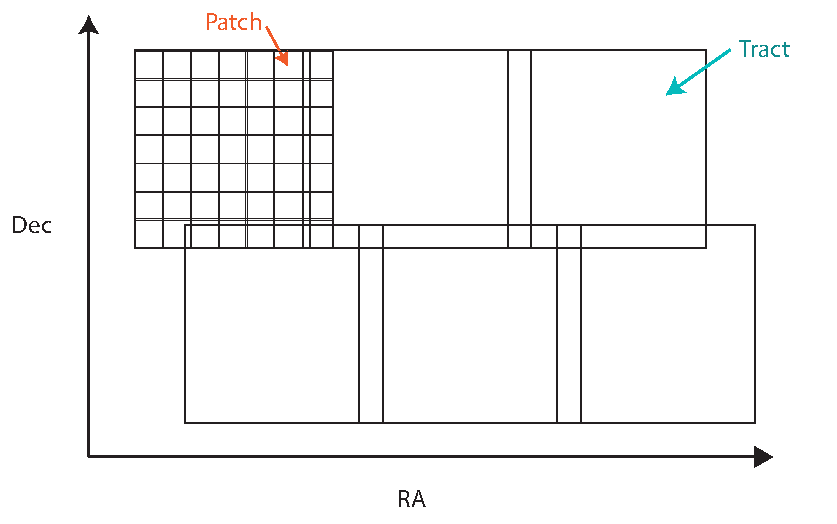
\includegraphics[width=0.6\textwidth]{results/tracts_and_patches.pdf} 
		
		\caption{A cartoon schematic of tracts and patches in the LSST on-sky data management tessellation The sky is divided intro overlapping tracts each $1.6^{\circ} \times 1.6^{\circ}$ Each tract is comprised of 49 overlapping patches. Patches are roughly the size of an individual LSSTCam CCD detector with dimensions of $13.7^{\prime} \times 13.7^{\prime}$ . }
		
		\label{fig:tractsandpatches}
	\end{figure}
	
	A patch is the smallest unit that will be handled by Rubin data processing pipeline. Template generation and subsequently image subtraction will be performed at the patch level. Figure \ref{fig:randompatch} shows an example the coverage in a single filter for a randomly selected patch chosen from the simulated Data Preview 0.2/DC2 \citep{2021ApJS..253...31L}  Year 1 Data Release image templates. The impact from the rotational dithers, spatial dithers, chip chaps, raft gaps, masked pixels at the detector edges, and saturated sources can be seen. An LSST patch will therefore not have uniform coverage across all of its pixels. This must be accounted for when estimating the Year 1 incremental template production rates. 
	
	\begin{figure}
		\centering
		\includegraphics[width=0.5\textwidth]{results/dc2-random_single_patch_year1_coadd_depth.pdf} 
		
		\caption{A representative patch randomly selected from the Rubin DP 0.2/DESC DC2  \citep{2021ApJS..253...31L} simulated data products Year 1 annual templates. 
			The extent of a single patch is $13.7 \times 13.7\ \si{arcmin}$.
			The colorbar reflects are how many visits went into that patch pixel.}
		
		\label{fig:randompatch}
	\end{figure}
	
	\subsection{\texttt{HEALPix} Sky Maps} 
	\label{sec:ITG}
	To track the Year 1 visits in a given area of sky suitable for making an incremental template and to identify which observations have sufficient template coverage to produce alerts and Solar System detections in Year 1, we place the sky onto a \texttt{HEALPix}\footnote{\url{http://healpix.sourceforge.net}} \citep[Hierarchical Equal Area isoLatitude Pixelization; ][]{2005ApJ...622..759G} map sliced into healpixels using an \verb|nside| factor that determines the resolution of each healpixel. It is too computationally expensive to consider incremental template generation at the individual patch pixel level as each patch has 16,810,000 pixels. Our best compromise is to instead focus on the patch as our smallest size element and use $\texttt{nside}=256$. This results in healpixels with a resolution of approximately $13.7\ \si{arcminutes}$ which is comparable in angular size to a patch. % 13.741946 arcmin  
	We note that this results in a \texttt{HEALPix} sky map grid that is close but is not exactly aligned with the patch/tract tessellation that the Rubin Observatory Data Management pipelines are using.  By using a healpixel resolution comparable to the patch size, we on average balance the problems of oversampling (large nside, high resolution healpixels) and undersampling (small nside, low resolution healpixels) when making our \texttt{HEALPix} incremental template coverage sky maps.
	
	\subsection{Year 1 Template Generation Timescales}
	\label{sec:timescales}
	As Year 1 of the survey progresses and images are taken according to the predefined survey strategy, sky coverage increases nightly. However, because of operational reasons (such as constraints on staffing and computational resources)  template production may not occur nightly in Year 1 but instead only on certain nights with some timescale (e.g.\ days - weeks). Template generation timescales have not yet been finalized by the Rubin Observatory Operations and Data Management Teams, but they are planning for a regular schedule (e.g. approximately monthly) \citep{DMTN-107,RTN-011}. We therefore explore a  range of template generation timescales ($\Delta t$): every 3, 7, 14, and 28 day intervals from the start of the simulated \baseline simulation. 
	
	\subsection{Requirements for Incremental Template Production}
	The individual image requirements and total number of observations needed to make suitable Year 1 templates in each filter has not yet been finalized by the Rubin Observatory Data Management Team \citep{DMTN-107,RTN-011}. On-sky tests with the commissioning camera (ComCam) and LSSTCam are needed. LSSTCam on-sky commissioning is expected to start in January 2025\footnote{The latest Rubin Observatory construction milestone schedule can be found at \url{https://www.lsst.org/about/project-status}}, at the time of of this paper's submission. In the meantime, we can make some reasonable assumptions based on the expected performance of the telescope and camera system. There are benefits and trade offs to balance for the image requirements applied to Year 1 template generation. This study is a first step in understanding the impact of incremental template generation,  so we elect to use very broad requirements for image quality. Further work will be needed needed to explore the full phase space of image requirements to optimize LSST Year 1 template building. 
	
	\subsubsection{Image Seeing and Depth Constraints}
	\label{sec:imageqa}
	Not every LSST observation taken in the first year of science operations should be combined to produce an image subtraction template. Observations taken in  poor seeing and/or bad photometic conditions should ideally be excluded. 
	On the other hand, if we are too restrictive with the image quality, then very few observations will meet our requirements making templates scarce in Year 1.  
	Using the values per visit reported in the \texttt{rubin\_sim} outputted pointing database, we evaluate the seeing quality  using the ``effective” full-width at half-maximum (FWHM), the FWHM of a single Gaussian describing the point spread function (PSF), (the \texttt{seeingFwhmEff} value) and image depth from the 5-$\sigma$ limiting magnitude. 
	We have no airmass constraints on incremental template generation. We also set no minimum time threhsold between suitable images as SSP only attempts to link sources that have moved within a night, so those Solar System object would be expected in most cases to move sufficiently far on the sky between the template building observations and future observations of the field to be distinguished as difference source by the Rubin image subtraction pipelines. 
	
	We impose broad image quality constraints to exclude the most outlying seeing and limiting magnitude observations. Each filter is evaluated separately, as each filter has different expected image depth and seeing distributions as shown in Tables \ref{tab:year1_image_seeing} and  \ref{tab:year1_image_depth}. 
	For a given healpix, filter $f$, and date in the survey, we look at all the relevant observations taken up to that point and  every observation $j$ that matches the following criteria will be considered to build the Year 1 template at that healpix location: 
	\begin{enumerate}
		\item seeing of frame $j$ /\texttt{min}(seeing of all available observations in filter $f$) $<$ 2
		\item (\texttt{max}(5-$\sigma$ limiting magnitude of all available observations in filter $f$) -  5-$\sigma$ limiting magnitude of frame $j$)$<$ 0.5
	\end{enumerate}
	This will reject the poorest quality images on average. There is a chance a healpix gets unlucky, and all the observations take up to that date are poor quality. In that case, if the seeing and depths do not vary significantly between the exposures, a Year 1 template would be still produced for that healpix. We look at the quality of the templates produced in Section \ref{sec:results}.
	
	%When generating templates in a given filter we select all visits that span a given healpixel and separate these visits into possible template/science images as described further in section \ref{sec:tracking_incremental_template_generation}.
	%We consider the seeing of these possible template images (\texttt{seeingFwhmEff}) and by divide by the benchmark seeing (the minimum seeing value; i.e.\ the least atmospheric distortion) of those images for this healpixel.
	%Only images with seeing within a factor \texttt{seeing ratio} = 2 of the benchmark are considered for template generation.
	%We then account for variation in the 5-$\sigma$ limiting magnitude depth of the possible template images, e.g.\ due to observations near the moon/giant planets with high sky brightness. \textbf{and cloudy images?}
	%The benchmark depth is the highest value (i.e.\ faintest magnitude) of the template images available for that healpixel in the given filter.
	%Images that have a \texttt{fiveSigmaDepth} which is brighter than the benchmark by \texttt{fiveSigmaDepth range} = 0.5 mag are not considered for template generation.
	%For reference we provide statistics on the seeing and depth of all \baseline visits (by filter) in Tables \ref{tab:year1_image_seeing} \& \ref{tab:year1_image_depth}.
	%It is particularly important to consider image quality for each filter separately, given the variation in typical depth and seeing for observations in different filters.
	%We note that we have not considered other constraints on template images such as a maximum airmass or a minimum time between images (e.g.\ slow moving Trans-Neptunian Objects (TNOs) may be present in templates within insufficient time gaps).
	%We have selected only basic constraints and have left detailed consideration of the effects of image quality on template creation to other work \textbf{(cite Eric's work?)}.
	%\textbf{We have recorded the mean seeing, mean depth and number of visits used to generate templates for each healpixel. Our constraints result in template images with seeing/depth typical for Year 1visits in that filter? ADD HISTOGRAMS. Emphasise the on-the-fly nature of image quality requirements - image quality constraint varies for each healpixel. We could make a bad template if all available images are trash but the scheduler is generally good - see histograms.
		%Note we don't consider the template quality after generation for the SSO MAF metrics - source artifacts can be dealt with by SSP pipeline (heliolinc) linking.}
	
	\begin{table}
		%	\tiny
		\centering
		\input{results/n_visits_4/df_year1_stats_seeing_first_year_baseline_v3_4_10yrs_db_noDD_noTwi.txt}
		\caption{
			Observation seeing statistics, per filter, reported for the ``effective" FWHM seeing for Year 1 of the \baseline cadence simulation (excluding low solar elongation twilight survey and DDF visits.)
		}
		\label{tab:year1_image_seeing}
	\end{table}
	
	\begin{table}
		%	\tiny
		\centering
		\input{results/n_visits_4/df_year1_stats_depth_first_year_baseline_v3_4_10yrs_db_noDD_noTwi.txt}
		\caption{
			Observation 5-$\sigma$ limiting magnitude (image depth) statistics, by filter, for Year 1 of the \baseline cadence simulation (excluding low solar elongation twilight survey and DDF visits).	
		}
		\label{tab:year1_image_depth}
	\end{table}
	
	\subsubsection{Number of Suitable Observations Used to Build a Year 1 Template}
	\label{sec:num_images}
	We also need to decide how many observations that meet our quality assurance criteria (described in Section \ref{sec:imageqa}) for template building should be combined to produce the Year 1 incremental templates at the patch level.  When considering healpixels with comparable angular size to patches, we note that there will be some cases when the overlap of images that lie within a given healpixel will not fill 100\% of the area (see the discussion in Section \ref{sec:tractsandpatches}), and the counted number of visits suitable for generating a template will be slightly overestimated or underestimated. We expect that across many healpixels these effects will on average balance out. We can also help mitigate this effect by picking a reasonable threshold on the number of suitable observations that must overlap with a patch (our sky map healpixel) to build a template such that at least 80-90$\%$ of the patch is covered. Recent Rubin Observatory technical notes propose that 3 good quality observations might be sufficient for making incremental templates \citep{DMTN-107,RTN-011}. The majority of the randomly selected DP0.2/DC2 patch in Figure \ref{fig:randompatch} is covered by at least 5 observations with more than $\sim$80$\%$ of the patch having at least 4 observation coverage. {We therefore add one more observation beyond the minimum proposed in \cite{DMTN-107} and \cite{RTN-011} and require 4 Year 1 observations per patch per filter that meet or exceed our seeing and image depth thresholds to ensure successful template building. % Need to update figs from n_visits_for_template = 3 to n_visits_for_template = 4 
		
		% See Lynne's figure in slack channel 16/08/2022, saved in this dir as lynne_image.png
		% make a figure with a nside = 256 healpixel plotted over lynne's very high resolution image
		% One will be able to see the variation of total counts within that the nside = 256 pixel
		%Vice versa, there may be cases where we have underestimated the number of images available for template generation within a particular however we expect that across many healpixels and over the course of Year 1 these effects will on average balance out. % think through how an underestimate comes up, see Mario post in slack
		%Furthermore, we note that our healpixel grid does not exactly align with the Rubin Observatory fixed skymap of patches.
		%However by using a healpixel resolution comparable to the patch size we on average balance the problems of oversampling (large nside, high resolution healpixels) and undersampling (small nside, low resolution healpixels) when assessing the various survey metrics.
		%Oversampling would overestimate the template area as we are assessing healpixels much smaller than the patches that the data processing pipeline will operate on.
		%Likewise undersampling leads to an underestimate of template coverage as smaller areas within the healpixels may have sufficient coverage for template generation.
		
		\subsection{Tracking Incremental Template Generation}
		\label{sec:tracking_incremental_template_generation}
		
		We step through the Year 1 simulated \texttt{rubin\_sim} \baseline pointing database in $\Delta t$ time intervals. At each template building session $n$, we iterate over all healpixels in our skymap and each of  the 6 LSST filters, selecting all visits that span a given healpixel and separating these visits into possible template building or science observations. We define $t_n$ as the time to generate incremental templates:
		\begin{equation}
			t_n= t_0+ \Delta t*n
		\end{equation}
		where $t_0$ is the start of the survey simulation's first observation. We perform this analysis varying $\Delta t$ to be  3, 7, 14, and  28 days (see Section \ref{sec:timescales}). Templates must be created separately for each filter. As such, we select all visits (with exposure start time of $t$)  in a given filter with $t<t_n$ that overlap the healpixel (aka patch). If there is no template already created, we look at all the observations taken up to that point, and we pick out the ones that match our image quality criteria (see Section \ref{sec:imageqa}). If at least $n=4$ images (see Section \ref{sec:num_images}) fitting these criteria are overlapping the healpixel then the template for that healpixel (aka patch) could have been generated. We then flag in our tracking database that the template has now been made at $t_n$ for that healpixel and filter combination, and record the number of nights since the first visit to the field which we will refer to as \texttt{deltaNight}. We assume that all subsequent observations in the given filter taken after $t_n$ that overlap that specific healpixel will be available for science processing and will be run through the Rubin Prompt Processing pipeplines. 
		
		We note that some healpixels may have $>$ 4 suitable observations available by the time of template generation and would likely have better depth/seeing and so be of higher quality. We do not adjust the 5-$\sigma$ limiting magnitude of an LSST observation based on the properties of its associated healpixels' templates. If the majority of the healpixel templates go to a much shallower depth than the observation it being subtracted from, there will be many bogus transient detections in addition to the real transient astrophysical sources and moving Solar System objects. We expect that  the SSP algorithms  will be able to handle this, and that these extra bogus transient detections will not pollute significantly SSP's moving object discoveries due to the constraint that the tracklets must be consistent with a heliocentric orbit over multiple days. The number of random false positive detections that could be combined in such a way to produce a decent heliocentric orbit fit, should be quite low. 
		
		% \textbf{N.B. we have considered just the visits within one healpixel but we keep the whole visit in our database, which could span several healpixels?}
		% The same visit would appear across several healpixels and would be removed/added to the database depending on the whether the healpixel had a template or not.
		% need to record the available visits for each healpixel? Keep a whole visit if >90% of its healpixels have templates?
		% Run the required metrics on the healpixels within the function, similar to Lynne
		% OR we run ``remove_no_templates" on a dataslice so the tests are calculated per healpixel but we record ``valid_ids" which is the unique number of ids.
		% Try keep all ids and count the number of times each visit appears. Multiply the counts by healpix area to get template coverage of whole visit.
		
		
		\subsection{Applying MAF Metrics}
		
		At this stage we are then able to use  MAF to run various metrics directly on the healpixels covering observations that had templates available. For example, we must sum the metric value (using the \texttt{Count} metric) for each healpixel to get the total number of visits/pairs, and we must find the minimum metric value when considering the first night when templates are available. We can also divide the summed healpixel area by the LSSTCam sky coverage (9.6 deg$^2$) so that we can determine the fractional template coverage of each visit (see Section \ref{sec:template_coverage}). 
		
		\begin{figure}
			\centering
			\begin{tabular}{c c c}
				\includegraphics[width=0.3\textwidth]{results/n_visits_4/first_year_baseline_v3_4_10yrs_db_noDD_noTwi_cum_baseline_u.pdf} &
				\includegraphics[width=0.3\textwidth]{results/n_visits_4/first_year_baseline_v3_4_10yrs_db_noDD_noTwi_cum_baseline_g.pdf} &
				\includegraphics[width=0.3\textwidth]{results/n_visits_4/first_year_baseline_v3_4_10yrs_db_noDD_noTwi_cum_baseline_r.pdf} \\
				\includegraphics[width=0.3\textwidth]{results/n_visits_4/first_year_baseline_v3_4_10yrs_db_noDD_noTwi_cum_baseline_i.pdf} &
				\includegraphics[width=0.3\textwidth]{results/n_visits_4/first_year_baseline_v3_4_10yrs_db_noDD_noTwi_cum_baseline_z.pdf} &
				\includegraphics[width=0.3\textwidth]{results/n_visits_4/first_year_baseline_v3_4_10yrs_db_noDD_noTwi_cum_baseline_y.pdf}
			\end{tabular}
			
			\caption{The cumulative healpixel area with templates for a given filter in Year 1 of the LSST.
				Each panel shows the results for the $ugrizy$ filters respectively.
				The area covered by the ideal baseline survey (assuming all templates exist at all times ) is shown by the black curve.
				The colored curves show the increase in area when template generation is considered ($\Delta t = 3, 7, 14, 28\ \si{days}$).
				The legend states the total area covered in that filter for the Year 1 baseline survey, and the fraction of that area reached for the different template timescales by the end of Year 1.
				The cumulative area is approximately related to the cumulative number of visits with templates given that each visit has an area of 9.6 deg$^2$ but that visit may not have 100\% template coverage.
				\textbf{rename y axis label to survey area?}
			}
			\label{fig:cum_baseline_filter}
			
		\end{figure}
		
		We also need to look beyond the individual healpixel (patch) level to the coverage at the LSSTCam FOV (tract) scale. If only a few patches in a given LSST exposure are able to be image subtracted, the moving objects will still be missed across most or all the frame. This is because the SSP detection algorithm must build tracklets, potential linkages in the same night from linear extrapolation using on-sky detections for two different observations of the same on-sky field at different times in a single night \citep{lsstMOPS,lsstSSP}.  SSP then takes the tracklets from the last 15 nights, and attempting to associate 3 tracklets onto a heliocentric orbit in order to identify new Solar System objects \citep{lsstMOPS,lsstSSP}. We therefore loop though the \texttt{rubin\_sim} pointing database, counting up the number of healpixels with available templates at the time of each LSST visit and adding this value a a column to the database. For discovering and characterizing Solar System objects we will only run MAF metrics on observations where the majority of the image area is available for template generation. We create a modified  \baseline pointing database removing visits where $<$ 90$\%$ of the healpixels within the visit's on-sky area have pre-made templates, and calculating a subset of MAF Solar System metrics using that redacted visit database.  We discuss the impact of varying the 90$\%$  coverage threshold in Section \ref{sec:results}.  
		
		
		% find the first not nan value when determining number and mean seeing/depth of template images
		
		
		
		
		\begin{deluxetable}{ll}
			\tablecaption{Solar System Discovery and Characterization MAF metrics used in this analysis.  \label{tab:metrics}}
			\tablehead{
				\colhead{Population } & \colhead{ Metrics}
			}
			\tabletypesize{\scriptsize}
			\startdata
			\multicolumn{2}{c}{Discovery Metrics} \\
			\hline
			\hline
			\multirow{2}{*}{PHAs} &  3 nightly pairs in 15 nights discovery completeness for $H\leq$ 16.0 \\
			& 3 nightly pairs in 15 nights discovery completeness for $H\leq$ 22.0 \\
			\hline
			\multirow{2}{*}{NEOs} & 3 nightly pairs in 15 nights discovery completeness for $H\leq$ 16.0 \\
			& 3 nightly pairs in 15 nights discovery completeness for $H\leq$ 22.0 \\
			\hline
			\multirow{2}{*}{MBAs} & 3 nightly pairs in 15 nights discovery completeness for $H\leq$ 16.0 \\
			& 3 nightly pairs in 15 nights discovery completeness for $H\leq$ 21.0 \\
			\hline
			\multirow{2}{*}{TNOs} & 3 nightly pairs in 15 nights discovery completeness for $H\leq$ 6.0 \\
			& 3 nightly pairs in 15 nights discovery completeness for $H\leq$ 8.0 \\
			\hline
			\multirow{2}{*}{OCC with $q\leq5$ au}   &  3 nightly pairs in 15 nights discovery completeness for $H\leq$ 8.0 \\
			& 3 nightly pairs in 15 nights discovery completeness for $H\leq$ 17.0\\
			\hline
			\multirow{2}{*}{OCCs  with $q\leq$ 20 au}   &  3 nightly pairs in 15 nights discovery completeness for $H\leq$ 8.0 \\
			& 3 nightly pairs in 15 nights discovery completeness  for $H\leq$ 12.0 \\ 
			\hline
			\multicolumn{2}{c}{Color-Light Curve Metrics} \\
			\hline
			\hline
			\multirow{2}{*}{PHAs} &  Fraction of $H$ = 16.0 with the equivalent of 40 SNR=5 detections or 10 SNR=20 detections per filter in $grizy$  \\
			&  Fraction of $H$ = 19.0 with the equivalent of 40 SNR=5 detections or 10 SNR=20 detections per filter in $grizy$  \\
			\hline
			\multirow{2}{*}{NEOs} & Fraction of $H$ = 16.0 with the equivalent of 40 SNR=5 detections or 10 SNR=20 detections per filter in $grizy$  \\
			&  Fraction of $H$ = 19.0 with the equivalent of 40 SNR=5 detections or 10 SNR=20 detections per filter in $grizy$  \\
			\hline
			\multirow{2}{*}{MBAs} &  Fraction of $H$ = 16.0 with the equivalent of 40 SNR=5 detections or 10 SNR=20 detections per filter in $grizy$  \\
			&  Fraction of $H$ = 18.0 with the equivalent of 40 SNR=5 detections or 10 SNR=20 detections per filter in $grizy$   \\
			\enddata
		\end{deluxetable}
		
		
		% \textbf{ss\_metrics: cite \cite{schwambTuningLegacySurvey2023} for the populations and metrics used! Very briefly summarise.}
		% \textbf{Focused on discovery as lightcurves will take 10yrs, colors as they may be available in year 1.}
		
		% \begin{enumerate}
			%     \item Input simulated survey pointings up to the template generation date
			%     \item Healpix slice
			%     \item Count observations of a given filter in each healpix
			%     \item Identify the first $n$ observations that meet the quality requirements
			%     \item Exclude pre-template images
			%     \item Exclude all visits with exposure time less than template generation date
			%     \item Repeat process for each template generation date (considering the cumulative number of observations)
			% \end{enumerate}
		
		
		
		\section{Results}
		\label{sec:results}
		
		% Some notes
		% https://docs.google.com/document/d/1T169SVAtmhsvc6t8C0ciYVhtzoWkk_St4D6PHSCpd4Q/edit?usp=sharing
		
		For each of our template generation timescales (3, 7, 14, and 28 days), we analyze both the tracked healpixel database and the redacted Year 1 observation pointing database described in \ref{sec:tracking_incremental_template_generation} calculating relevant statistics and MAF metrics.  
		
		\subsection{Template Quality and Number of Observations Used in Template Production}
		
		In Figure Set \ref{fig:template_image_histograms_tscale}, we plot, per filter, a histogram of the number of observations used to build each template and the resulting  distribution of mean limiting magnitudes and the mean observed seeing values that are used to produce each of the incremental templates per patch. At the patch level, our template generation algorithm only produces a template each generation time step if there are at least four or more consistent quality images and a template had not been previously generated on an earlier day. We find that across all time steps we tested, the majority of templates are created with four or five observations. At longer template generation time steps, an increasing number of templates are created from  $>$ 4 observations given the abundance of images of available goes up with longer gaps between template building days. Overall,  the distribution of mean seeing and mean image depth are consistent across all template building timescales and are reproduce the same distribution of image quality values across the entire set of Year 1 observations (listed in Tables \ref{tab:year1_image_seeing} and \ref{tab:year1_image_depth}). These results are not necessarily surprising given the Rubin scheduler is designed to make decisions on which filter to observed is based in part on the observing conditions to ensure that the science requirements \citep{lsstSRD} for the LSST image quality per filter in individual and co-added observations are met. We have applied very broad requirements on image quality for this paper. We note that implementing more stringent thresholds for which LSST observations can contribute to  Year 1 template production will likely see more  differences between the template generation timescales and the overall properties of Year 1 observations.
		
		\begin{figure}
			\centering
			\begin{tabular}{c c c}
				
				%		\includegraphics[width=0.25\textwidth]{results/n_visits_4/histograms_templates_tscale/hist_first_year_baseline_v3_4_10yrs_db_noDD_noTwi_doALLTemplateMetrics_reduceNTemplate_u_noDD_noTwi.pdf} &
				%\includegraphics[width=0.25\textwidth]{results/n_visits_4/histograms_templates_tscale/hist_first_year_baseline_v3_4_10yrs_db_noDD_noTwi_doALLTemplateMetrics_reduceSeeingTemplate_u_noDD_noTwi.pdf} &
				%\includegraphics[width=0.25\textwidth]{results/n_visits_4/histograms_templates_tscale/hist_first_year_baseline_v3_4_10yrs_db_noDD_noTwi_doALLTemplateMetrics_reduceDepthTemplate_u_noDD_noTwi.pdf} \\
				
				%		\includegraphics[width=0.25\textwidth]{results/n_visits_4/histograms_templates_tscale/hist_first_year_baseline_v3_4_10yrs_db_noDD_noTwi_doALLTemplateMetrics_reduceNTemplate_g_noDD_noTwi.pdf} &
				%\includegraphics[width=0.25\textwidth]{results/n_visits_4/histograms_templates_tscale/hist_first_year_baseline_v3_4_10yrs_db_noDD_noTwi_doALLTemplateMetrics_reduceSeeingTemplate_g_noDD_noTwi.pdf} &
				%\includegraphics[width=0.25\textwidth]{results/n_visits_4/histograms_templates_tscale/hist_first_year_baseline_v3_4_10yrs_db_noDD_noTwi_doALLTemplateMetrics_reduceDepthTemplate_g_noDD_noTwi.pdf} \\
				
				\includegraphics[width=0.3\textwidth]{results/n_visits_4/histograms_templates_tscale/hist_first_year_baseline_v3_4_10yrs_db_noDD_noTwi_doALLTemplateMetrics_reduceNTemplate_r_noDD_noTwi.pdf} &
				\includegraphics[width=0.3\textwidth]{results/n_visits_4/histograms_templates_tscale/hist_first_year_baseline_v3_4_10yrs_db_noDD_noTwi_doALLTemplateMetrics_reduceSeeingTemplate_r_noDD_noTwi.pdf} &
				\includegraphics[width=0.3\textwidth]{results/n_visits_4/histograms_templates_tscale/hist_first_year_baseline_v3_4_10yrs_db_noDD_noTwi_doALLTemplateMetrics_reduceDepthTemplate_r_noDD_noTwi.pdf} \\
				
			\end{tabular}
			\caption{
				\textbf{separate by filter.}
				\textbf{left panel uses a curve of the histogram to highlight differences}
				\textbf{Make a AAS multifigure to show different filters.}
				\textbf{Add a table with the summary template generation stats? In appendix?}
			}
			\label{fig:template_image_histograms_tscale}
		\end{figure}
		
		
		
		
		% \textbf{Jamie: Show some results for the MAF healpixel analysis and give some numbers:}
		% - Area of the the sky with templates/fraction of survey footprint with templates as a function of time (figures \ref{fig:cumFrac_baseline}, \ref{fig:cumFrac_deltaNight}). % combine my plot with Lynne's, will only have a datapoint on each template generation night. Use her method as a baseline assuming template generation every night
		% % Can also use an estimate based on the redacted database
		
		% - Number of visits with templates (compare to number in baseline). % skymap and histogram
		
		% - Number of visits with pairs and templates - required for moving object detection. % skymap and histogram
		
		% - First night when template is available: compare our results to Lynne's method (when templates are continuously generated). % Use Lynne's results directly or rerun our code with template generation every night, might be slow?
		
		% - Table of percentage sky visits and number of visits with/without templates, i.e. the percentage of images not being searched and not available for alert generation!
		% \\
		
		
		\subsection{On-Sky Template Coverage (Patch Scale)}
		\label{sec:template_coverage}
		
		(See Figure \ref{fig:fractional_template_coverage}).
		
		Our analysis shows that the requirements of template generation during Year 1of the LSST greatly reduces the area of the sky over which detections can be made via difference imaging.
		This is shown in Figure \ref{fig:cum_baseline_filter}, where we have plotted the cumulative sky area with templates as determined on a healpixel basis using the MAF metric (\verb|reduceCount|) described in section \ref{sec:methods}.
		We could not consider the number of visits with templates directly; each visit contains multiple healpixels ($\sim183$ for nside 256) and not all healpixels within a visit necessarily have templates due to the overlap of previous dithered visits (Figures \ref{fig:randompatch} \& \ref{fig:fractional_template_coverage}). % add Lynne high res snapshot figure?
		% reorder figures to get fig:fractional_template_coverage in numerical order?
		In Figure \ref{fig:cum_baseline_filter} the cumulative healpixel area is the non-unique area with templates, i.e.\ we have summed the area with templates for each visit.
		Therefore this parameter is closely related to the number of visits with templates (if one were to account for the differing fractional template area per visit, Figure \ref{fig:fractional_template_coverage}).
		We have considered each filter separately and included the cumulative healpixel area that would have been covered in the baseline simulation if templates existed for the full sky (black curve in Figure \ref{fig:cum_baseline_filter}).
		All filters lag behind the baseline; the $rizy$ filters only achieve \red{74-80\%} of the baseline area for a 3 day template generation timescale.
		The $u$ and $g$ filters have achieve noticeably lower cumulative healpixel areas than the other filters \red{(41\% and 52\% respectively for $\Delta t = 3\ \si{d}$)}.
		We note that as the template generation timescale is increased the cumulative healpixel area also decreases, with some filters experiencing greater decreases than others.
		The cumulative healpixel area for filters $uizy$ decreases by \red{$4-7\%$} as $\Delta t = 3 \rightarrow 28\ \si{d}$, whereas the drop for filters $gr$ is larger at \red{$10 - 12 \%$}.
		
		These trends are also shown in Figure \ref{fig:cumFrac_baseline}, where we again plot the cumulative healpixel area with templates  but now normalised by the total baseline area in that filter.
		Here each panel shows the results for the different template generation timescales and we can compare each filter directly; in all cases the $ug$ filters lag behind the others.
		This implies that the observing strategy for the $ug$ filters in \baseline (i.e.\ cadence/re-visit time) is more sensitive to the delays added when template generation is accounted for.
		The decrease in survey sky area when template generation is considered (Figures \ref{fig:cum_baseline_filter} \& \ref{fig:cumFrac_baseline}) implies that there will be a corresponding reduction in the number of transient detections in the prompt data products (including alerts of high priority targets, e.g.\ Solar System PHAs and ISOs) during Year 1of LSST. 
		\\
		
		
		
		\begin{figure}
			\centering
			
			\includegraphics[width=0.8\textwidth]{results/n_visits_4/histograms/hist_first_year_baseline_v3_4_10yrs_db_noDD_noTwi_CountMetric_doAllTemplateMetrics_reduceCount_all_noDD_noTwi.pdf}
			
			\caption{
				Histograms showing the sky area ($y$ axis) for which healpixels have $0, 1, 2...$ visits ($x$ axis) at the end of Year 1considering all filters.
				We show the histogram distribution for the baseline where template generation is assumed (blue).
				The distributions when template generation is required ($\Delta t = 3, 7, 14, 28\ \si{d}$) are denoted by the coloured lines.
			}
			\label{fig:template_baseline_all}
		\end{figure}
		
		\begin{figure}
			\centering
			\begin{tabular}{c c}
				\includegraphics[width=0.4\textwidth]{results/n_visits_4/histograms/hist_first_year_baseline_v3_4_10yrs_db_noDD_noTwi_CountMetric_doAllTemplateMetrics_reduceCount_u_7_noDD_noTwi.pdf} &
				\includegraphics[width=0.4\textwidth]{results/n_visits_4/histograms/hist_first_year_baseline_v3_4_10yrs_db_noDD_noTwi_CountMetric_doAllTemplateMetrics_reduceCount_g_7_noDD_noTwi.pdf} \\
				\includegraphics[width=0.4\textwidth]{results/n_visits_4/histograms/hist_first_year_baseline_v3_4_10yrs_db_noDD_noTwi_CountMetric_doAllTemplateMetrics_reduceCount_r_7_noDD_noTwi.pdf} &
				\includegraphics[width=0.4\textwidth]{results/n_visits_4/histograms/hist_first_year_baseline_v3_4_10yrs_db_noDD_noTwi_CountMetric_doAllTemplateMetrics_reduceCount_i_7_noDD_noTwi.pdf} \\
				\includegraphics[width=0.4\textwidth]{results/n_visits_4/histograms/hist_first_year_baseline_v3_4_10yrs_db_noDD_noTwi_CountMetric_doAllTemplateMetrics_reduceCount_z_7_noDD_noTwi.pdf} &
				\includegraphics[width=0.4\textwidth]{results/n_visits_4/histograms/hist_first_year_baseline_v3_4_10yrs_db_noDD_noTwi_CountMetric_doAllTemplateMetrics_reduceCount_y_7_noDD_noTwi.pdf} \\
			\end{tabular}
			\caption{
				Histograms of sky area as a function of number of visits per healpixel (similar to figure \ref{fig:template_baseline_all}) but each panel shows the results for the $ugrizy$ filters.
				For clarity we show only the results for the baseline and $\Delta t = 7\ \si{d}$.
				\textbf{NB shift of roughly 3-6 visits from baseline, try ask for these extra visits in commissioning? Mention in conclusions.}
				\textbf{Make a AAS multifigure to show different tscales.}
			}
			\label{fig:template_baseline_histograms}
		\end{figure}
		
		
		\begin{figure}
			\centering
			\begin{tabular}{c c}
				\includegraphics[width=0.4\textwidth]{results/n_visits_4/skymaps/skymap_first_year_baseline_v3_4_10yrs_db_noDD_noTwi_tscale-28_nside-256_doAllTemplateMetrics_reduceCount_u_noDD_noTwi.pdf} &
				\includegraphics[width=0.4\textwidth]{results/n_visits_4/skymaps/skymap_first_year_baseline_v3_4_10yrs_db_noDD_noTwi_tscale-28_nside-256_doAllTemplateMetrics_reduceCount_g_noDD_noTwi.pdf} \\
				\includegraphics[width=0.4\textwidth]{results/n_visits_4/skymaps/skymap_first_year_baseline_v3_4_10yrs_db_noDD_noTwi_tscale-28_nside-256_doAllTemplateMetrics_reduceCount_r_noDD_noTwi.pdf} &
				\includegraphics[width=0.4\textwidth]{results/n_visits_4/skymaps/skymap_first_year_baseline_v3_4_10yrs_db_noDD_noTwi_tscale-28_nside-256_doAllTemplateMetrics_reduceCount_i_noDD_noTwi.pdf} \\
				\includegraphics[width=0.4\textwidth]{results/n_visits_4/skymaps/skymap_first_year_baseline_v3_4_10yrs_db_noDD_noTwi_tscale-28_nside-256_doAllTemplateMetrics_reduceCount_z_noDD_noTwi.pdf} &
				\includegraphics[width=0.4\textwidth]{results/n_visits_4/skymaps/skymap_first_year_baseline_v3_4_10yrs_db_noDD_noTwi_tscale-28_nside-256_doAllTemplateMetrics_reduceCount_y_noDD_noTwi.pdf} \\
			\end{tabular}
			\caption{Skymaps showing the total number of visits with templates, per healpixel (nside = 256), at the end of year 1, assuming a template generation timescale of 28 days. Each panel shows the results for the $ugrizy$ filters.
				Compare to figure \ref{fig:baseline_skymaps} for the baseline number of visits per pixel at the end of year 1.
			}
			\label{fig:template_skymaps_tscale-28}
		\end{figure}
		
		
		The need to accumulate sufficient past visits to generate templates will naturally introduce a time delay to when difference image detections start to appear in the LSST alert stream.
		This time delay is captured by the MAF \verb|deltaNight| metric, as shown in Figure \ref{fig:cumFrac_deltaNight}.
		This metric measures the number of nights between the first visit (in a given filter) to a particular healpixel and the night on which its template (in that filter) was generated.
		This therefore removes the bias of which area of the sky is the current focus of the survey. %, e.g.\ the WFD will tend to prioritise visits at low airmass and so preferentially images the sky directly overhead which will change over time \textbf{(see lynne animation \texttt{baseline\_v3.2\_10yrs\_first})}.
		Figure \ref{fig:cumFrac_deltaNight} shows that as $\Delta t$ is decreased, the time delay to create a template is also decreased.
		In this figure the cumulative fraction of footprint area refers to the unique on-sky area planned for Year 1of the survey in that filter; therefore the figure indicates the rate at which the template coverage increases.
		The \texttt{deltaNight} metric in Figure \ref{fig:cumFrac_deltaNight} is more closely modulated by the choice of $\Delta t$ than the \texttt{reduceCount} metric in Figure \ref{fig:cum_baseline_filter}, this is particularly clear for the $u$ filter results.
		As $\Delta t$ is increased from $3 \rightarrow 28\ \si{d}$ the time between first visit and template generation increases from \red{$5 \rightarrow 27\ \si{d}$ for $25\%$} of the footprint area.
		This effect is most pronounced for low values of \texttt{deltaNight} when it is less likely for there to be sufficient re-visits to a given field to generate templates. 
		As $\texttt{deltaNight}\rightarrow 90\ \si{days}$ all filters have started to converge and we see that $\sim 90\%$ of each filter's survey footprint has templates, as $90\ \si{days}$ is several times greater than the template generation timescales considered here. 
		% Lynne on slack: The g band lag .. maybe also related to bright time influencing the cadence? We pair g band with u band images as well as r band images, and it's fairly blue, so we do tend to take more g band visits near dark time. There are also just fewer g band visits. Looking at the distribution on the sky, it does look a bit like dark time / bright time kinds of things to me.
		\\
		
		\begin{figure}
			\begin{center}
				\begin{interactive}{animation}{animation.mp4}
				\end{interactive}
%				\includegraphics[width=0.5\columnwidth]{results/first_year_baseline_v3_4_10yrs_db_noDD_noTwi_tscale-3_nside-256_CountMetric_r_and_night_lt_84_and_note_not_like_DD_and_note_not_like_twilight_HEAL.pdf}
				\includegraphics[width=0.5\columnwidth]{results/baseline_v3_4_tscale-3_CountMetric_84.pdf}
				\caption{Snapshot from a video animation of the sky coverage over time in \baseline observing strategy where incremental templates are produced in Year 1.  The animation steps through in intervals over the first year of the simulated LSST displaying the cumulative number of on-sky visits in the $r$ filter. The plots are centered on $\alpha$=0 and $\delta$=0. Right ascension and declination lines are marked every 30$^\circ$.} (An animation of this figure is available.)  Note to Editor/Reviewer: The animation is currently available from (\href{https://uoe-my.sharepoint.com/:v:/g/personal/jrobin10_ed_ac_uk/Ef0X-FVuKAhNtJtvRQiyPDMBi-5ypVqPowcvGSMqsr9PZw?nav=eyJyZWZlcnJhbEluZm8iOnsicmVmZXJyYWxBcHAiOiJPbmVEcml2ZUZvckJ1c2luZXNzIiwicmVmZXJyYWxBcHBQbGF0Zm9ybSI6IldlYiIsInJlZmVycmFsTW9kZSI6InZpZXciLCJyZWZlcnJhbFZpZXciOiJNeUZpbGVzTGlua0NvcHkifX0&e=ysWV8t}{temp link 1} \label{animation:baseline}
			\end{center}
		\end{figure}
		
		\begin{figure}
			\begin{center}
				\begin{interactive}{animation}{animation3d.mp4}
				\end{interactive}
%				\includegraphics[width=0.5\columnwidth]{results/n_visits_4/first_year_baseline_v3_4_10yrs_db_noDD_noTwi_tscale-3_nside-256_doAllTemplateMetrics_reduceCount_r_and_night_lt_84_and_note_not_like_DD_and_note_not_like_twilight_HEAL.pdf}
				\includegraphics[width=0.5\columnwidth]{results/n_visits_4/baseline_v3_4_tscale-3_reduceCount_84.pdf}
				\caption{Snapshot from a video animation of the sky coverage over time in \baseline observing strategy in the case where templates are produced incrementally every 3 days over the first year of the simulated survey  The animation steps through in intervals over the first year of the simulated LSST displaying the cumulative number of on-sky visits in the $r$ filter. The plots are centered on $\alpha$=0 and $\delta$=0. Right ascension and declination lines are marked every 30$^\circ$.} (An animation of this figure is available.) Note to Editor/Reviewer: The animation is currently available from (\href{https://uoe-my.sharepoint.com/:i:/g/personal/jrobin10_ed_ac_uk/EUN-c34vnEhGqAQQM5mUa6IBH9gxRnU3ufP9h5sCSHjz2w?e=O73p7P}{temp link 2} \label{animation:3dsays}
			\end{center}
		\end{figure}
		
		As mentioned previously, the on-sky extent of each visit will lie across multiple healpixels over which the MAF metrics are being calculated.
		For example at a resolution of nside = 256 a LSST visit of 9.6 square degrees will cover approximately 183 healpixels.
		Not all healpixels within a visit footprint will necessarily have an available template at the time of exposure, due to the dithering of past exposures.
		Therefore in addition to the metrics described above we record the number of constituent healpixels with templates for each visit.
		Figure \ref{fig:fractional_template_coverage} shows a histogram of the fraction of healpixels with templates within a visit, for all visits in Year 1of \baseline.
		The large spike at zero indicates the visits that had zero \% template coverage and so could not have generated any alerts.
		\textbf{The template coverage is $>90\%$ for FRAC of visits during year 1.}
		Note that the small number of visits with coverage $>100\%$ arises due to healpixels which include only part of the visit footprint (the footprint does not align perfectly with the healpixel grid and we may overestimate area due to healpixel resolution).
		% Jamie Note: fraction of the TOTAL baseline survey area (area includes repeat observations, i.e. equivalent to total number of observations)
		
		We also include animated figures showing the cumulative skymap visit coverage in Year 1for the \baseline simulation (\href{https://uoe-my.sharepoint.com/:i:/g/personal/jrobin10_ed_ac_uk/EYo4E-4aDIhJlVPfUr-r7bEBHzUUZG5EYAiqQjVAz1u-dg?e=ar4exU}{temp link 1}) and the various template generation simulations (\href{https://uoe-my.sharepoint.com/:i:/g/personal/jrobin10_ed_ac_uk/EWMteDuQN6pKsADBES4XXWUBO9ArRd2cQGFxMVo1IrsGmg?e=iMlYe2}{temp link 2}).
		\textbf{Both show just the $r$ filter and the template simulation is for $\Delta t = 3\ \si{d}$}
		These animations highlight the time lag when template generation must be considered, and the patchier coverage when visits without templates are rejected.
		
		\begin{figure}
			\centering
			\begin{tabular}{c c}
				\includegraphics[width=0.4\textwidth]{results/n_visits_4/skymaps/skymap_first_year_baseline_v3_4_10yrs_db_noDD_noTwi_tscale-7_nside-256_doAllTemplateMetrics_reduceCount_u_noDD_noTwi.pdf} &
				\includegraphics[width=0.4\textwidth]{results/n_visits_4/skymaps/skymap_first_year_baseline_v3_4_10yrs_db_noDD_noTwi_tscale-7_nside-256_doAllTemplateMetrics_reduceCount_g_noDD_noTwi.pdf} \\
				\includegraphics[width=0.4\textwidth]{results/n_visits_4/skymaps/skymap_first_year_baseline_v3_4_10yrs_db_noDD_noTwi_tscale-7_nside-256_doAllTemplateMetrics_reduceCount_r_noDD_noTwi.pdf} &
				\includegraphics[width=0.4\textwidth]{results/n_visits_4/skymaps/skymap_first_year_baseline_v3_4_10yrs_db_noDD_noTwi_tscale-7_nside-256_doAllTemplateMetrics_reduceCount_i_noDD_noTwi.pdf} \\
				\includegraphics[width=0.4\textwidth]{results/n_visits_4/skymaps/skymap_first_year_baseline_v3_4_10yrs_db_noDD_noTwi_tscale-7_nside-256_doAllTemplateMetrics_reduceCount_z_noDD_noTwi.pdf} &
				\includegraphics[width=0.4\textwidth]{results/n_visits_4/skymaps/skymap_first_year_baseline_v3_4_10yrs_db_noDD_noTwi_tscale-7_nside-256_doAllTemplateMetrics_reduceCount_y_noDD_noTwi.pdf} \\
			\end{tabular}
			\caption{Skymaps showing the total number of visits with templates, per healpixel (nside = 256), at the end of year 1, assuming a template generation timescale of 7 days. Each panel shows the results for the $ugrizy$ filters.
				Compare to figure \ref{fig:baseline_skymaps} for the baseline number of visits per pixel at the end of year 1.
			}
			\label{fig:template_skymaps_tscale-7}
		\end{figure}
		
		\begin{figure}
			\centering
			\begin{tabular}{c c}
				
				\includegraphics[width=0.34\textwidth]{results/n_visits_4/skymaps/skymaps_delta_first_year_baseline_v3_4_10yrs_db_noDD_noTwi_CountMetric_doAllTemplateMetrics_reduceCount_u_7_noDD_noTwi} &				
				\includegraphics[width=0.34\textwidth]{results/n_visits_4/skymaps/skymaps_delta_first_year_baseline_v3_4_10yrs_db_noDD_noTwi_CountMetric_doAllTemplateMetrics_reduceCount_u_28_noDD_noTwi} \\
				
				\includegraphics[width=0.34\textwidth]{results/n_visits_4/skymaps/skymaps_delta_first_year_baseline_v3_4_10yrs_db_noDD_noTwi_CountMetric_doAllTemplateMetrics_reduceCount_g_7_noDD_noTwi} &				
				\includegraphics[width=0.34\textwidth]{results/n_visits_4/skymaps/skymaps_delta_first_year_baseline_v3_4_10yrs_db_noDD_noTwi_CountMetric_doAllTemplateMetrics_reduceCount_g_28_noDD_noTwi} \\
				
				\includegraphics[width=0.34\textwidth]{results/n_visits_4/skymaps/skymaps_delta_first_year_baseline_v3_4_10yrs_db_noDD_noTwi_CountMetric_doAllTemplateMetrics_reduceCount_r_7_noDD_noTwi} &			
				\includegraphics[width=0.34\textwidth]{results/n_visits_4/skymaps/skymaps_delta_first_year_baseline_v3_4_10yrs_db_noDD_noTwi_CountMetric_doAllTemplateMetrics_reduceCount_r_28_noDD_noTwi} \\
				
				\includegraphics[width=0.34\textwidth]{results/n_visits_4/skymaps/skymaps_delta_first_year_baseline_v3_4_10yrs_db_noDD_noTwi_CountMetric_doAllTemplateMetrics_reduceCount_i_7_noDD_noTwi} &				
				\includegraphics[width=0.34\textwidth]{results/n_visits_4/skymaps/skymaps_delta_first_year_baseline_v3_4_10yrs_db_noDD_noTwi_CountMetric_doAllTemplateMetrics_reduceCount_i_28_noDD_noTwi} \\
				
				
				\includegraphics[width=0.34\textwidth]{results/n_visits_4/skymaps/skymaps_delta_first_year_baseline_v3_4_10yrs_db_noDD_noTwi_CountMetric_doAllTemplateMetrics_reduceCount_z_7_noDD_noTwi} &			
				\includegraphics[width=0.34\textwidth]{results/n_visits_4/skymaps/skymaps_delta_first_year_baseline_v3_4_10yrs_db_noDD_noTwi_CountMetric_doAllTemplateMetrics_reduceCount_z_28_noDD_noTwi} \\
				
				\includegraphics[width=0.34\textwidth]{results/n_visits_4/skymaps/skymaps_delta_first_year_baseline_v3_4_10yrs_db_noDD_noTwi_CountMetric_doAllTemplateMetrics_reduceCount_y_7_noDD_noTwi} &				
				\includegraphics[width=0.34\textwidth]{results/n_visits_4/skymaps/skymaps_delta_first_year_baseline_v3_4_10yrs_db_noDD_noTwi_CountMetric_doAllTemplateMetrics_reduceCount_y_28_noDD_noTwi} \\
				
			\end{tabular}
			\caption{Skymaps (with healpixels nside = 256) per filter of the  difference between total number of visits with templates in Year 1 and the ideal \baseline. \textbf{Left:} Template generation timescale $\Delta t = 7 \si{d}$.  \textbf{Right:} Template generation timescale $\Delta t = 28 \si{d}$. Most of the sky has templates generated very quickly so the loss is only the 4 visits used to produce the templates, but 7 days template production timescales is less patchy and has more healpixels with a 4 image loss.    
			}
			\label{fig:template_skymaps_delta-7_28days}
		\end{figure}
		
		
		\subsection{Solar System Discovery and Color Light-Curve Metrics}
		\label{sec:sso_metrics}
		
		Now that we know the template coverage for each visit we can analysis the Year 1 Solar System discovery metrics, considering only visits that had a fractional template coverage of $\geq 90 \%$ (Figure \ref{fig:fractional_template_coverage}).
		\textbf{Why 90\%?}
		These metrics operate by generating a sample of orbits from a particular dynamical population and assigning properties such as absolute magnitude and surface color from the assumed distributions.
		The simulated object ephemerides are generated for every visit time and any objects that could have been detected during that visit are recorded.
		We calculate the fraction of the sample population that meets a specific metric criteria, which provides an estimate for the full population we expect the survey to characterise.
		This methodology and details of the metrics analysed are described further in \cite{schwambTuningLegacySurvey2023}.
		In this work we have focused on a Solar System object discovery metric, and a color characterisation metric.
		
		Figure \ref{fig:temp_gen_discovery_metrics} shows the results for the discovery metric of objects that have had 3 pairs of detections over a 15 night period.
		We have considered a range of dynamical populations \textbf{(MBA, NEO, PHA, TNO, OCC\_r5, OCC\_r20)} as the different orbits and physical properties of these populations have a strong influence on discovery and characterisation.
		Each test population consists of 5000 objects randomly sampled from an appropriate synthetic population \cite[see Section 2.2 of][for more details]{schwambTuningLegacySurvey2023}.
		We present the metric results of each template generation timescale relative to the default \baseline survey where the presence of templates is implicitly assumed (i.e.\ all visits are capable of making detections).
		\textbf{drop in discovery rate. dependent on population, e.g. slow moving TNOs vs.\ faster moving MBAs?}
		
		Likewise we in Figure \ref{fig:temp_gen_colour_metrics} we present the results for the characterisation metric describing how many objects in the sample for which at least 4 colors are obtained from the grizy filters.
		We follow the analysis of \cite{schwambTuningLegacySurvey2023} and only consider colors for the MBA, NEO and PHA populations.
		\textbf{TNOs and OCCs do not get any colors when templates are considered.}
		\textbf{drop in color measurements}
		
		In Figure \ref{fig:completeness_over_time} we consider in more detail how the cumulative completeness (that is the fraction of objects in the sample that have been discovered) increase as a function of survey time.
		
		The results of these MAF Solar System metrics provide a more direct estimate of the effects of template generation on Solar System science, than simply looking at the on sky area with templates as considered previously.
		We can clearly see that the requirements of template generation leads to large drops in the discovery and measurement of colors for the dynamical populations investigated.
		If we compare to the analysis in \cite{schwambTuningLegacySurvey2023}, they compared different survey strategies and stated that a $\pm5\%$ variation in a given metric would be acceptable (relative to the baseline survey at the time).
		However these results shows drops of up to \red{50\%} in discovery (Figure \ref{fig:temp_gen_discovery_metrics}).
		Furthermore the time delay introduced by generating templates (Figure \ref{fig:cumFrac_deltaNight}) is present in Figure \ref{fig:completeness_over_time} \textbf{(plus additional delay?)}.
		Altogether these results highlight that ``real-time'' Solar System discoveries in Year 1 will be severely affected by template generation.
		
		\subsection{Additional tests}
		\label{sec:additional_tests}
		
		\textbf{reduce the template image quality requirements to generate worse templates but faster. e.g. 4 rather than 3 visits required for templates. See also Meg's email about Figure \ref{fig:randompatch}.}
		
		\textbf{Is $g$ filter observations the limiting factor? Compare results to the override-g simulations where template generation has been ignored for all $g$ filter observations.}
		\\
		
		The results of section \ref{sec:template_coverage} show that the $u$ and $g$ filters always lag behind the other filters when template generation is considered (Figure \ref{fig:cumFrac_baseline}).
		Of these two filters, the redder $g$ band will play a greater role in the study of SSOs; this has been accounted for in \baseline where $g$ band observations extend into the NES whereas $u$ band does not.
		Therefore, we conducted a brief investigation into whether the additional lag in $g$ band visits was negatively affecting the discovery (i.e.\ pairs where at least one is visit $g$ band) and characterisation of SSOs (where a color measurement is relative to $g$ band).
		
		To do this we repeated our template generation simulation of section \ref{sec:methods} for \baseline, but we assumed that templates were always available for $g$ band visits (all other filters required incremental template generation).
		We tested the largest and smallest timescales; $\Delta t = 3, 28\ \si{d}$.
		We then calculated the SSO discovery and color metrics described in section \ref{sec:sso_metrics}, now using all $g$ band visits and visits in other filters that had $\geq90\%$ template coverage.
		
		\textbf{findings...}
		We find that the SSO metrics are improved by \textbf{a few percent} when all $g$ visits are assumed to have templates.
		The relative increase in the discovery and color metrics is greater when $\Delta t$ is smaller.
		The relatively minor improvement in the metrics shows that while improved template generation for the lagging $g$ band can help, we are still limited by the lack of templates in the other filters (which have more visits than $g$ in year 1).
		This highlights that improving SSO discovery and characterisation while performing incremental template generation during Year 1 is a difficult problem with many factors to consider.
		However, if templates can be generated rapidly (on the order of days) it may be possible to make minor changes to the planned schedule in order to increase the rate at which the sky is covered and reduce the delay introduced by template generation and improve the Year 1 SSO metrics.
		
		
		%%% figures - add code to generate in overleaf repo (avoid sub-dirs!)
		% share the simulation repo with Mario
		
		% include some sky maps, nvisits, deltaNight?
		
		% cumulative fraction of baseline area - equivalent to n_visits(t)/n_visits_total 
		\begin{figure}
			\centering
			\begin{tabular}{c c}
				\includegraphics[width=0.3\textwidth]{results/n_visits_4/first_year_baseline_v3_4_10yrs_db_noDD_noTwi_cumFrac_baseline_3.pdf} &
				\includegraphics[width=0.3\textwidth]{results/n_visits_4/first_year_baseline_v3_4_10yrs_db_noDD_noTwi_cumFrac_baseline_7.pdf} \\
				\includegraphics[width=0.3\textwidth]{results/n_visits_4/first_year_baseline_v3_4_10yrs_db_noDD_noTwi_cumFrac_baseline_14.pdf} &
				\includegraphics[width=0.3\textwidth]{results/n_visits_4/first_year_baseline_v3_4_10yrs_db_noDD_noTwi_cumFrac_baseline_28.pdf}
			\end{tabular}
			\caption{ An alternative to Figure \ref{fig:cum_baseline_filter}, where now we plot the cumulative area covered in a particular filter as a fraction of the total baseline area in that filter.
				In each panel we show the result for a particular template generation timescale (7, 14, 28 days) and the color of each curve indicates the filter (ugrizy).
				\textbf{Furthermore the legend provides the fractional cumulative area at the end of year one for each filter.}
			}
			\label{fig:cumFrac_baseline}
		\end{figure}
		
		
		% cumulative fraction of footprint area vs deltaNight - equivalent to the rate at which full coverage is reached
		\begin{figure}
			\centering
			\begin{tabular}{c c c}
				\includegraphics[width=0.3\textwidth]{results/n_visits_4/first_year_baseline_v3_4_10yrs_db_noDD_noTwi_doAllTemplateMetrics_reduceDeltaNight_u.pdf} &
				\includegraphics[width=0.3\textwidth]{results/n_visits_4/first_year_baseline_v3_4_10yrs_db_noDD_noTwi_doAllTemplateMetrics_reduceDeltaNight_g.pdf} &
				\includegraphics[width=0.3\textwidth]{results/n_visits_4/first_year_baseline_v3_4_10yrs_db_noDD_noTwi_doAllTemplateMetrics_reduceDeltaNight_r.pdf} \\
				\includegraphics[width=0.3\textwidth]{results/n_visits_4/first_year_baseline_v3_4_10yrs_db_noDD_noTwi_doAllTemplateMetrics_reduceDeltaNight_i.pdf} &
				\includegraphics[width=0.3\textwidth]{results/n_visits_4/first_year_baseline_v3_4_10yrs_db_noDD_noTwi_doAllTemplateMetrics_reduceDeltaNight_z.pdf} &
				\includegraphics[width=0.3\textwidth]{results/n_visits_4/first_year_baseline_v3_4_10yrs_db_noDD_noTwi_doAllTemplateMetrics_reduceDeltaNight_y.pdf}
			\end{tabular}
			\caption{Plots showing the cumulative fraction of the Year 1 survey footprint area \textbf{i.e.\ the unique on-sky area covered by that filter in the Year 1 survey)} against \texttt{deltaNight}, which is the number of days between the first visit to a healpixel and the night at which a template was generated.
				% Jamie Note: This is the unique sky area covered in each filter
				Each panel shows the results for a different filter (ugrizy).
				The $x$ axis is limited to show a maximum $\texttt{deltaNight}=90\ \si{d}$ to highlight the timescale over which there is the greatest change.
				\textbf{footprint area refers to unique on sky area for a given filter in year 1.}
			}
			\label{fig:cumFrac_deltaNight}
		\end{figure}
		
		% redacted database fractional template coverage figure
		\begin{figure}
			\centering
			\includegraphics[width=0.5\textwidth]{results/n_visits_4/fractional_template_coverage_first_year_baseline_v3_4_10yrs_db_noDD_noTwi.pdf}
			\caption{Histogram of the fractional template coverage for all Year 1 visits, which is determined from the number of healpixels within the visit footprint with templates.
				Results are shown for the \baseline cadence simulation, assuming a range of template generation timescales.
				\textbf{The peak at zero consists mainly of the images used to make the templates (Table \ref{tab:year1_N_visits_templates}).}
			}
			\label{fig:fractional_template_coverage}
		\end{figure}
		
		\begin{table}
			%	\tiny
			\centering
			\input{results/n_visits_4/df_N_temp_first_year_baseline_v3_4_10yrs_db_noDD_noTwi.txt}
			\caption{
				The number of visits that were used to generate templates for each filter for different template generation timescales $\Delta t$.
				\textbf{This is an approximate number of visits, calculated as number of visits used to generate the first template in all healpixels times healpixel area divided by the camera footprint area.}
			}
			\label{tab:year1_N_visits_templates}
		\end{table}
		
		% moving object metrics for faint/bright dynamical populations:
		
		% relative detection loss
		\begin{figure}
			\centering
			\begin{tabular}{c c}
				\includegraphics[width=0.5\textwidth]{results/n_visits_4/baseline_v3_4_n_visits_4_discovery_metric_bright.pdf} &
				\includegraphics[width=0.5\textwidth]{results/n_visits_4/baseline_v3_4_n_visits_4_discovery_metric_faint.pdf}
			\end{tabular}
			\caption{Here we show the results of running the Rubin Solar System body discovery metrics on a redacted year 1 visit database with templates (\baseline, using only visits with $\geq 90\%$ template coverage).
				We analyse the metric for discoveries requiring 3 detection pairs over the space of 15 nights, considering several dynamical populations (MBA, NEO, PHA, TNO, OCC\_r5 and OCC\_r20) which indicated by color and marker shape.
				The results of this metric for the tested template generation timescales (3, 7, 14, 28 days) are given relative to the results for the \baseline year 1 survey in which templates are assumed to already exist.
				The left panel shows the discovery metric for the ``bright'' objects in each population (low $H$) and the right panel shows the ``faint'' objects (high $H$).
				\textbf{Metric, bright and faint defined in table \ref{tab:metrics}.}
			}
			\label{fig:temp_gen_discovery_metrics}
		\end{figure}
		
		% colour metrics
		\begin{figure}
			\centering
			\begin{tabular}{c c}
				\includegraphics[width=0.5\textwidth]{results/n_visits_4/baseline_v3_4_n_visits_4_colour_metric_bright.pdf} &
				\includegraphics[width=0.5\textwidth]{results/n_visits_4/baseline_v3_4_n_visits_4_colour_metric_faint.pdf}
			\end{tabular}
			\caption{Similar to Figure \ref{fig:temp_gen_discovery_metrics} but now showing the metric value (relative to the baseline) of Solar System bodies for which at least 4 colors can be measured from the ugrizy filters.
				\textbf{3 and 7 d the same for faint MBAs?}
				\textbf{Metric, bright and faint defined in table \ref{tab:metrics}.}
			}
			\label{fig:temp_gen_colour_metrics}
		\end{figure}
		
		% completeness over time
		\begin{figure}
			\centering
			\begin{tabular}{c c c}
				\includegraphics[width=0.3\textwidth]{results/n_visits_4/DiscoveryTime_MBA_first_year_baseline_v3_4_10yrs_db_n_visits_4_noDD_noTwi.pdf} &
				\includegraphics[width=0.3\textwidth]{results/n_visits_4/DiscoveryTime_NEO_first_year_baseline_v3_4_10yrs_db_n_visits_4_noDD_noTwi.pdf} &
				\includegraphics[width=0.3\textwidth]{results/n_visits_4/DiscoveryTime_PHA_first_year_baseline_v3_4_10yrs_db_n_visits_4_noDD_noTwi.pdf} \\
				\includegraphics[width=0.3\textwidth]{results/n_visits_4/DiscoveryTime_TNO_first_year_baseline_v3_4_10yrs_db_n_visits_4_noDD_noTwi.pdf} &
				\includegraphics[width=0.3\textwidth]{results/n_visits_4/DiscoveryTime_OCC_r5_first_year_baseline_v3_4_10yrs_db_n_visits_4_noDD_noTwi.pdf} &
				\includegraphics[width=0.3\textwidth]{results/n_visits_4/DiscoveryTime_OCC_r20_first_year_baseline_v3_4_10yrs_db_n_visits_4_noDD_noTwi.pdf} \\
			\end{tabular}
			\caption{Plots showing the discovery completeness of each population during year 1 of the survey, i.e.\ the cumulative fraction of objects that have been discovered as a function of time.
				The line colors distinguish the \baseline survey where template generation has been implicitly assumed and the simulations in which template generation has been considered (for template generation timescales of 3, 7, 14, 28 days).
				The various panels display results for the different dynamical populations considered in this work: MBA, NEO, PHA, TNO, OCC\_r5, OCC\_r20.
				\textbf{share y axis of pairs? rerun ss metrics and replot}
				\textbf{show 7 and 28 - rest in supplemental online figure set }
				\textbf{Metrics, bright and faint described in table \ref{tab:metrics}.}
			}
			\label{fig:completeness_over_time}
		\end{figure}
		
		\section{Summary and Conclusions}
		\label{sec:summary_conclusions}
		
		We have investigated the impact of incremental template generation in Year 1 of the LSST using the \texttt{rubin\_sim} simulated \baseline observing strategy and associated LSST MAF metrics, assuming that the Rubin scheduler executes the baseline strategy. Focusing on Solar System discovery and characterization metrics, we used MAF to simulate the effects of generating templates in the first year of the survey, by counting the number of visits in each healpixel of the sky and establishing when the criteria for template generation has been met, assuming no significant contribution of template-grade observations during the commissioning of Rubin Observatory and excluding the DDFs and low Solar elongation twilight survey observations. Using a 3, 7, 14, and 28 day template building cadence coupled with a 90$\%$ coverage threshold for each LSST observation, we summarize our findings below:
		
		\begin{itemize}
			\item Early template generation is preferred. The sooner templates are generated, the closer the performance to the idealized \baseline observing strategy's real-time discovery rates. This is because more observations become available for nightly prompt processing at shorter template production timescales. 
			\item Across all the metrics we evaluated, a monthly template strategy performs the worst. A 3-day/7-day turnaround time for template production provides the most opportunities to identify transient sources in the LSST observations in real-time and results in more uniform coverage. 
			\item Over all production timescales explored, incremental template coverage in $g$-band and $u$-band significantly lag behind the other filters due to the small number of observations in these filters during first year of the survey. 
			\item Due to the reduced number of visits planned in the NES (compared to the WFD), the majority of the observations taken in Year 1 especially in the $g$ filter go into templates building and will not be able to be searched by the nightly Prompt Processing pipelines for transient sources and moving Solar System objects. 
			\item We expect it will take approximately 2 months from the start of the survey to build sufficient numbers of templates in multiple filters for nightly Solar System discoveries by SSP to begin. 
			\item For both Solar System discoverability and the color light-curve metrics, the shorter template generation timescales perform better. 
			\item The discovery metrics across all small body populations simulated have more than a \red{20$\%$} decrease compared the perfect Year 1 baseline metrics. The MBA discovery metrics are impacted the most with a drop greater than \red{30$\%$} for the larger ($H \leq$ 16) objects and greater than \red{45$\%$} for the smaller asteroids ($H \leq$ 21).  
			\item In general, the discoverability of smaller (and typically fainter) objects are impacted more significantly by Year 1 template generation than larger (typically brighter) objects. 
			\item The inner Solar System color light-curve metrics are significantly more impacted than the discovery  metrics. There is a drop of more than \red{75$\%$} compared to the perfect Year 1 baseline, with longer template generation timescales performing worse for the majority of MBA, NEO, and PHA populations. 
		\end{itemize}
		
		Without modifications to the baseline (\baseline) Year 1 observing strategy, there will be some LSST observations with suitable templates made as the survey progresses to allow image subtraction within 60 s of the shutter closing, enabling the Rubin Prompt Processing and SSP pipelines to run and generate nightly Solar System discoveries/alerts. But there is a non-negligible hit to real-time detection and characterization of Solar System small bodies. The change in MAF metrics is much higher than the 5$\%$ difference from the baseline strategy deemed acceptable in \cite{schwambTuningLegacySurvey2023}'s evaluation of cadence parameters for optimizing LSST Solar System System science. For each small body population simulated, the larger objects are impacted less because they are typically brighter in apparent magnitude and thus more likely to be detectable in most or all of the LSST observations that they are present in. Smaller (and typically fainter) objects require more chances to be able to detect them, and thus are impacted more by incremental template generation strategies. 
		The discovery metrics are impacted less than color light-curve metrics because it takes many more observations with pre-generated templates (10-20 good signal-to-noise ratio detections per filter in $griz$) to measure good surface colors compared to the 6 pairs of nightly detections over 14 days required for linking by SSP. 
		Locations within the main part of the LSST footprint (WFD) receive at most \red{$\sim$7-12} $g$ observations over the year compared to the redder filters which have \red{$\sim$13-20} observations visits per filter (see Figure \ref{fig:baseline_skymaps}), so the color light-curve metric is highly sensitive to the number of repeat visits across the LSST footprint that Prompt Processing and SSP pipelines can run on, especially in the case of $g$ template production. 
		The drop in the discovery metrics is likely effected by the lack of $g$ templates, as $g$ is typically paired with the $r$ filter, there are likely nightly pairs. 
		Exploring options for boosting Year 1 template production in $g$ will be the first step to improve the number of nightly pairs searchable each night for moving objects. 
		
		We have focused in this paper on Solar System metrics, but there are some parallels that can be drawn to the discovery of astrophysical transients using the Rubin alert stream. The alert stream will only be populated from LSST observations when suitable template building observations covering the majority of the image's on-sky footprint already exists for the given observation's filter. We see a non-negligible impact to the the Solar System discovery metrics, which require 3 nightly pairs of observations within 14 days. Therefore, we expect there will be reductions in real-time astrophysical transient detections in Year 1 and the associated Year 1 MAF metrics, as it will take take several observations to identify the characteristic brightening in a transient source's light curve consistent with a supernovae or tidal disruption event. Additionally, the variable stars and astrophysical transients community has advocated for different filters to be used in the LSST nightly pairs \citep{2019PASPpresto} with $g$ and $u$ bands paired with the $r$ \citep{SCOC_Report_1, SCOC_Report_2} to explore color evolution over a night. With the bluer filters trailing in template coverage compared to the redder filters, there will be likely be less chances to discover and spectroscopically characterize fast-changing explosive transients.  Further work is needed to explore the full impact of incremental template generation on opportunities to discover and rapidly follow-up different classes of astrophysical transients during Year 1 of the LSST. 
		
		This work is a first step towards understanding the expected discovery yields and discovery output from the LSST Prompt Processing data products and Rubin alert stream in Year 1 operations. 
		The Rubin Observatory operations and data management teams, have yet to settle on an incremental template strategy \citep{DMTN-107,RTN-011}. 
		Based on our analysis, we strongly recommend that they explore the possibility of generating templates on weekly or shorter timescales.  
		We have assumed that there is no significant contribution to Year 1 templates from commissioning and that the \baseline observing strategy is executed with no modifications to prioritize incremental template building. We have also assumed that the first four suitable observations of a given patch are used to produce templates with generous image quality constraints. 
		Further analysis is needed to explore more sophisticated strategies and differing requirements for incremental template generation. The Year 1 LSST observing cadence is also likely not optimized for incremental template generation.  
		Further \texttt{rubin\_sim} simulations are needed to examine if and how the Rubin scheduler can be tuned to maximize template production over the first year without significantly impacting the 10-year outputs of the survey. 
		Strategies to boost the $g$ and $u$ template production rates in Year 1 should also be studied. It is important for the community and the SCOC to explore other modifications to the Year 1 observing cadence  that may significantly boost template production  across all filters, such as allocating a small amount of observing time earmarked for obtaining Year 1 template building. 
		Currently the LSST survey strategy employs two back-to-back 15s exposures (snaps) per visit that are combined to produce a single LSST observation. The SCOC and Rubin Observatory are considering moving to one 30s snap. If it is possible to transition to 1 snap, some of the additional observing time could go into template building observations in specific filters or parts of the footprint like the galactic plane and NES that have less total visits than the WFD footprint. If it is not possible for the LSST to switch to 1 snap per visit or allocate the freed up on-sky time, other alternatives to boost the number of observations in the NES in Year 1 should be explored. It is vital that studies exploring the possible parameter space for incremental template generation within the LSST observing strategy and its impact on the LSST 10-year and Year 1 MAF metrics be completed well before the start of Rubin on-sky commissioning with LSSTCam (currently expected to start in January 2025). 
		This will provide an opportunity to optimize the Year 1 observing strategy for alert production while giving the community the most time to initiate follow-up preparations for the start of the LSST with the best picture of what Year 1 nightly outputs of the survey will look like.
		
		\begin{acknowledgments}
			
			This work was supported in part by the LSST Discovery Alliance Enabling Science grants program, the B612 Foundation, the University of Washington's DiRAC (Data-intensive Research in Astrophysics and Cosmology) Institute, the Planetary Society, and Karman+ through generous support of the LSST Solar System Readiness Sprints. MES was supported by the UK Science Technology Facilities Council (STFC) grants ST/V000691/1 and ST/X001253/1. MES also acknowledges support from LSST Discovery Alliance through grant [2023-SFF-LFI-01-Schwamb], and this support was provided by the generosity of Eric and Wendy Schmidt by recommendation of the Schmidt Futures program.
			
			This research has made use of NASA's Astrophysics Data System Bibliographic Services.Some of the results in this paper have been derived using the \texttt{healpy} and \texttt{HEALPix} packages
			
			Data Access:  Data used in this paper are openly available from the Vera C. Rubin Observatory Construction Project and Operations Teams. The rubin$\_$sim LSST cadence simulation databases used in this work are publicly available from \cite{v3.4sims}. \textbf{update to v3.4 ref.}
			
		\end{acknowledgments}
		
		\facility{Rubin}
		
		\software{healpy \citep{2005ApJ...622..759G,Zonca2019}, LSST Metrics Analysis Framework \citep[MAF,][]{2014SPIE.9149E..0BJ}, rubin$\_$sim \citep{2014SPIE.9150E..14C, 2014SPIE.9150E..15D, 2017arXiv170804058L, 2019AJ....157..151N, jones_r_lynne_2020_4048838}}
		
		\section*{Author Contributions}
		
		\appendix
		\section{Additional Plots}
		\label{appendix:A}
		
		In this appendix we provide additional figures covering simulations of all template generation timescales and results for each filter.
		\textbf{Describe figures.}
		
		
		\begin{table}
			\centering
			\input{results/n_visits_4/df_frac_coverage_first_year_baseline_v3_4_10yrs_db_noDD_noTwi.txt}
			\caption{Table showing the total pixel area with templates (in a given filter) at the end of year 1, as a fraction of the baseline total pixel area.
				This is approximately equivalent to the fraction of visits that have templates at the end of Year 1 (we did not count visits directly as most visits have less than $100\%$ template coverage as shown in Figure \ref{fig:fractional_template_coverage}).
				These values are the same as the fractional area at night 365 shown in Figures \ref{fig:cum_baseline_filter}, \ref{fig:cumFrac_baseline}.}
			\label{tab:template_pixel_area}
		\end{table}
		
		
		% baseline skymaps
		
		
		% \begin{figure}
			% 	\centering
			% 	\begin{tabular}{c c}
				% 		\includegraphics[width=0.4\textwidth]{results/n_visits_4/skymaps/skymap_first_year_baseline_v3_4_10yrs_db_noDD_noTwi_tscale-3_nside-256_doAllTemplateMetrics_reduceCount_u_noDD_noTwi.pdf} &
				% 		\includegraphics[width=0.4\textwidth]{results/n_visits_4/skymaps/skymap_first_year_baseline_v3_4_10yrs_db_noDD_noTwi_tscale-3_nside-256_doAllTemplateMetrics_reduceCount_g_noDD_noTwi.pdf} \\
				% 		\includegraphics[width=0.4\textwidth]{results/n_visits_4/skymaps/skymap_first_year_baseline_v3_4_10yrs_db_noDD_noTwi_tscale-3_nside-256_doAllTemplateMetrics_reduceCount_r_noDD_noTwi.pdf} &
				% 		\includegraphics[width=0.4\textwidth]{results/n_visits_4/skymaps/skymap_first_year_baseline_v3_4_10yrs_db_noDD_noTwi_tscale-3_nside-256_doAllTemplateMetrics_reduceCount_i_noDD_noTwi.pdf} \\
				% 		\includegraphics[width=0.4\textwidth]{results/n_visits_4/skymaps/skymap_first_year_baseline_v3_4_10yrs_db_noDD_noTwi_tscale-3_nside-256_doAllTemplateMetrics_reduceCount_z_noDD_noTwi.pdf} &
				% 		\includegraphics[width=0.4\textwidth]{results/n_visits_4/skymaps/skymap_first_year_baseline_v3_4_10yrs_db_noDD_noTwi_tscale-3_nside-256_doAllTemplateMetrics_reduceCount_y_noDD_noTwi.pdf} \\
				% 	\end{tabular}
			% 	\caption{Skymaps showing the total number of visits with templates, per healpixel (nside = 256), at the end of year 1, assuming a template generation timescale of 3 days. Each panel shows the results for the $ugrizy$ filters.
				% 		Compare to figure \ref{fig:baseline_skymaps} for the baseline number of visits per pixel at the end of year 1.
				% 	}
			% 	\label{fig:template_skymaps_tscale-3}
			% \end{figure}
		
		\begin{figure}
			\centering
			\begin{tabular}{c c}
				\includegraphics[width=0.4\textwidth]{results/n_visits_4/skymaps/skymap_first_year_baseline_v3_4_10yrs_db_noDD_noTwi_tscale-7_nside-256_doAllTemplateMetrics_reduceCount_u_noDD_noTwi.pdf} &
				\includegraphics[width=0.4\textwidth]{results/n_visits_4/skymaps/skymap_first_year_baseline_v3_4_10yrs_db_noDD_noTwi_tscale-7_nside-256_doAllTemplateMetrics_reduceCount_g_noDD_noTwi.pdf} \\
				\includegraphics[width=0.4\textwidth]{results/n_visits_4/skymaps/skymap_first_year_baseline_v3_4_10yrs_db_noDD_noTwi_tscale-7_nside-256_doAllTemplateMetrics_reduceCount_r_noDD_noTwi.pdf} &
				\includegraphics[width=0.4\textwidth]{results/n_visits_4/skymaps/skymap_first_year_baseline_v3_4_10yrs_db_noDD_noTwi_tscale-7_nside-256_doAllTemplateMetrics_reduceCount_i_noDD_noTwi.pdf} \\
				\includegraphics[width=0.4\textwidth]{results/n_visits_4/skymaps/skymap_first_year_baseline_v3_4_10yrs_db_noDD_noTwi_tscale-7_nside-256_doAllTemplateMetrics_reduceCount_z_noDD_noTwi.pdf} &
				\includegraphics[width=0.4\textwidth]{results/n_visits_4/skymaps/skymap_first_year_baseline_v3_4_10yrs_db_noDD_noTwi_tscale-7_nside-256_doAllTemplateMetrics_reduceCount_y_noDD_noTwi.pdf} \\
			\end{tabular}
			\caption{Skymaps showing the total number of visits with templates, per healpixel (nside = 256), at the end of year 1, assuming a template generation timescale of 7 days. Each panel shows the results for the $ugrizy$ filters.
				Compare to figure \ref{fig:baseline_skymaps} for the baseline number of visits per pixel at the end of year 1.
			}
			\label{fig:template_skymaps_tscale-7_figure_set}
		\end{figure}
		
		\begin{figure}
			\centering
			\begin{tabular}{c c}
				\includegraphics[width=0.4\textwidth]{results/n_visits_4/skymaps/skymap_first_year_baseline_v3_4_10yrs_db_noDD_noTwi_tscale-14_nside-256_doAllTemplateMetrics_reduceCount_u_noDD_noTwi.pdf} &
				\includegraphics[width=0.4\textwidth]{results/n_visits_4/skymaps/skymap_first_year_baseline_v3_4_10yrs_db_noDD_noTwi_tscale-14_nside-256_doAllTemplateMetrics_reduceCount_g_noDD_noTwi.pdf} \\
				\includegraphics[width=0.4\textwidth]{results/n_visits_4/skymaps/skymap_first_year_baseline_v3_4_10yrs_db_noDD_noTwi_tscale-14_nside-256_doAllTemplateMetrics_reduceCount_r_noDD_noTwi.pdf} &
				\includegraphics[width=0.4\textwidth]{results/n_visits_4/skymaps/skymap_first_year_baseline_v3_4_10yrs_db_noDD_noTwi_tscale-14_nside-256_doAllTemplateMetrics_reduceCount_i_noDD_noTwi.pdf} \\
				\includegraphics[width=0.4\textwidth]{results/n_visits_4/skymaps/skymap_first_year_baseline_v3_4_10yrs_db_noDD_noTwi_tscale-14_nside-256_doAllTemplateMetrics_reduceCount_z_noDD_noTwi.pdf} &
				\includegraphics[width=0.4\textwidth]{results/n_visits_4/skymaps/skymap_first_year_baseline_v3_4_10yrs_db_noDD_noTwi_tscale-14_nside-256_doAllTemplateMetrics_reduceCount_y_noDD_noTwi.pdf} \\
			\end{tabular}
			\caption{Skymaps showing the total number of visits with templates, per healpixel (nside = 256), at the end of year 1, assuming a template generation timescale of 14 days. Each panel shows the results for the $ugrizy$ filters.
				Compare to figure \ref{fig:baseline_skymaps} for the baseline number of visits per pixel at the end of year 1.
			}
			\label{fig:template_skymaps_tscale-14}
		\end{figure}
		
		\begin{figure}
			\centering
			\begin{tabular}{c c}
				\includegraphics[width=0.4\textwidth]{results/n_visits_4/skymaps/skymap_first_year_baseline_v3_4_10yrs_db_noDD_noTwi_tscale-28_nside-256_doAllTemplateMetrics_reduceCount_u_noDD_noTwi.pdf} &
				\includegraphics[width=0.4\textwidth]{results/n_visits_4/skymaps/skymap_first_year_baseline_v3_4_10yrs_db_noDD_noTwi_tscale-28_nside-256_doAllTemplateMetrics_reduceCount_g_noDD_noTwi.pdf} \\
				\includegraphics[width=0.4\textwidth]{results/n_visits_4/skymaps/skymap_first_year_baseline_v3_4_10yrs_db_noDD_noTwi_tscale-28_nside-256_doAllTemplateMetrics_reduceCount_r_noDD_noTwi.pdf} &
				\includegraphics[width=0.4\textwidth]{results/n_visits_4/skymaps/skymap_first_year_baseline_v3_4_10yrs_db_noDD_noTwi_tscale-28_nside-256_doAllTemplateMetrics_reduceCount_i_noDD_noTwi.pdf} \\
				\includegraphics[width=0.4\textwidth]{results/n_visits_4/skymaps/skymap_first_year_baseline_v3_4_10yrs_db_noDD_noTwi_tscale-28_nside-256_doAllTemplateMetrics_reduceCount_z_noDD_noTwi.pdf} &
				\includegraphics[width=0.4\textwidth]{results/n_visits_4/skymaps/skymap_first_year_baseline_v3_4_10yrs_db_noDD_noTwi_tscale-28_nside-256_doAllTemplateMetrics_reduceCount_y_noDD_noTwi.pdf} \\
			\end{tabular}
			\caption{Skymaps showing the total number of visits with templates, per healpixel (nside = 256), at the end of year 1, assuming a template generation timescale of 28 days. Each panel shows the results for the $ugrizy$ filters.
				Compare to figure \ref{fig:baseline_skymaps} for the baseline number of visits per pixel at the end of year 1.
			}
			\label{fig:template_skymaps_tscale-28-fig-set}
		\end{figure}
		
		\begin{figure}
			\centering
			\begin{tabular}{c c c c}
				% \includegraphics[width=0.2\textwidth]{results/n_visits_4/skymaps/skymaps_delta_first_year_baseline_v3_4_10yrs_db_noDD_noTwi_CountMetric_doAllTemplateMetrics_reduceCount_u_3_noDD_noTwi} &
				\includegraphics[width=0.2\textwidth]{results/n_visits_4/skymaps/skymaps_delta_first_year_baseline_v3_4_10yrs_db_noDD_noTwi_CountMetric_doAllTemplateMetrics_reduceCount_u_7_noDD_noTwi} &				\includegraphics[width=0.2\textwidth]{results/n_visits_4/skymaps/skymaps_delta_first_year_baseline_v3_4_10yrs_db_noDD_noTwi_CountMetric_doAllTemplateMetrics_reduceCount_u_14_noDD_noTwi} &
				\includegraphics[width=0.2\textwidth]{results/n_visits_4/skymaps/skymaps_delta_first_year_baseline_v3_4_10yrs_db_noDD_noTwi_CountMetric_doAllTemplateMetrics_reduceCount_u_28_noDD_noTwi} \\
				
				% \includegraphics[width=0.2\textwidth]{results/n_visits_4/skymaps/skymaps_delta_first_year_baseline_v3_4_10yrs_db_noDD_noTwi_CountMetric_doAllTemplateMetrics_reduceCount_g_3_noDD_noTwi} &
				\includegraphics[width=0.2\textwidth]{results/n_visits_4/skymaps/skymaps_delta_first_year_baseline_v3_4_10yrs_db_noDD_noTwi_CountMetric_doAllTemplateMetrics_reduceCount_g_7_noDD_noTwi} &				\includegraphics[width=0.2\textwidth]{results/n_visits_4/skymaps/skymaps_delta_first_year_baseline_v3_4_10yrs_db_noDD_noTwi_CountMetric_doAllTemplateMetrics_reduceCount_g_14_noDD_noTwi} &
				\includegraphics[width=0.2\textwidth]{results/n_visits_4/skymaps/skymaps_delta_first_year_baseline_v3_4_10yrs_db_noDD_noTwi_CountMetric_doAllTemplateMetrics_reduceCount_g_28_noDD_noTwi} \\
				
				% \includegraphics[width=0.2\textwidth]{results/n_visits_4/skymaps/skymaps_delta_first_year_baseline_v3_4_10yrs_db_noDD_noTwi_CountMetric_doAllTemplateMetrics_reduceCount_r_3_noDD_noTwi} &
				\includegraphics[width=0.2\textwidth]{results/n_visits_4/skymaps/skymaps_delta_first_year_baseline_v3_4_10yrs_db_noDD_noTwi_CountMetric_doAllTemplateMetrics_reduceCount_r_7_noDD_noTwi} &				\includegraphics[width=0.2\textwidth]{results/n_visits_4/skymaps/skymaps_delta_first_year_baseline_v3_4_10yrs_db_noDD_noTwi_CountMetric_doAllTemplateMetrics_reduceCount_r_14_noDD_noTwi} &
				\includegraphics[width=0.2\textwidth]{results/n_visits_4/skymaps/skymaps_delta_first_year_baseline_v3_4_10yrs_db_noDD_noTwi_CountMetric_doAllTemplateMetrics_reduceCount_r_28_noDD_noTwi} \\
				
				% \includegraphics[width=0.2\textwidth]{results/n_visits_4/skymaps/skymaps_delta_first_year_baseline_v3_4_10yrs_db_noDD_noTwi_CountMetric_doAllTemplateMetrics_reduceCount_i_3_noDD_noTwi} &
				\includegraphics[width=0.2\textwidth]{results/n_visits_4/skymaps/skymaps_delta_first_year_baseline_v3_4_10yrs_db_noDD_noTwi_CountMetric_doAllTemplateMetrics_reduceCount_i_7_noDD_noTwi} &				\includegraphics[width=0.2\textwidth]{results/n_visits_4/skymaps/skymaps_delta_first_year_baseline_v3_4_10yrs_db_noDD_noTwi_CountMetric_doAllTemplateMetrics_reduceCount_i_14_noDD_noTwi} &
				\includegraphics[width=0.2\textwidth]{results/n_visits_4/skymaps/skymaps_delta_first_year_baseline_v3_4_10yrs_db_noDD_noTwi_CountMetric_doAllTemplateMetrics_reduceCount_i_28_noDD_noTwi} \\
				
				% \includegraphics[width=0.2\textwidth]{results/n_visits_4/skymaps/skymaps_delta_first_year_baseline_v3_4_10yrs_db_noDD_noTwi_CountMetric_doAllTemplateMetrics_reduceCount_z_3_noDD_noTwi} &
				\includegraphics[width=0.2\textwidth]{results/n_visits_4/skymaps/skymaps_delta_first_year_baseline_v3_4_10yrs_db_noDD_noTwi_CountMetric_doAllTemplateMetrics_reduceCount_z_7_noDD_noTwi} &				\includegraphics[width=0.2\textwidth]{results/n_visits_4/skymaps/skymaps_delta_first_year_baseline_v3_4_10yrs_db_noDD_noTwi_CountMetric_doAllTemplateMetrics_reduceCount_z_14_noDD_noTwi} &
				\includegraphics[width=0.2\textwidth]{results/n_visits_4/skymaps/skymaps_delta_first_year_baseline_v3_4_10yrs_db_noDD_noTwi_CountMetric_doAllTemplateMetrics_reduceCount_z_28_noDD_noTwi} \\
				
				% \includegraphics[width=0.2\textwidth]{results/n_visits_4/skymaps/skymaps_delta_first_year_baseline_v3_4_10yrs_db_noDD_noTwi_CountMetric_doAllTemplateMetrics_reduceCount_y_3_noDD_noTwi} &
				\includegraphics[width=0.2\textwidth]{results/n_visits_4/skymaps/skymaps_delta_first_year_baseline_v3_4_10yrs_db_noDD_noTwi_CountMetric_doAllTemplateMetrics_reduceCount_y_7_noDD_noTwi} &				\includegraphics[width=0.2\textwidth]{results/n_visits_4/skymaps/skymaps_delta_first_year_baseline_v3_4_10yrs_db_noDD_noTwi_CountMetric_doAllTemplateMetrics_reduceCount_y_14_noDD_noTwi} &
				\includegraphics[width=0.2\textwidth]{results/n_visits_4/skymaps/skymaps_delta_first_year_baseline_v3_4_10yrs_db_noDD_noTwi_CountMetric_doAllTemplateMetrics_reduceCount_y_28_noDD_noTwi} \\
				
			\end{tabular}
			\caption{Skymaps showing the \textbf{difference} between total number of visits with templates, per healpixel (nside = 256) at the end of year 1, between the baseline and template generation tests. Each row shows the results for a $ugrizy$ filter.
				Each column is a different template generation timescale ($\Delta t = 3, 7, 14, 28\ \si{d}$).
				\textbf{replot this for $\Delta t = 3$ but with columns for baseline skymap, template skymap and then difference?}
				\textbf{focus on 7 and 28 - figure set of a column for each timescale.}
			}
			\label{fig:template_skymaps_delta-full}
		\end{figure}
		
		\begin{figure}
			\centering
			\begin{tabular}{c c c c}
				\raisebox{.4\height}{\includegraphics[width=0.2\textwidth]{results/n_visits_4/skymaps_cutout/skymaps_cutout_first_year_baseline_v3_4_10yrs_db_noDD_noTwi_nside-256_CountMetric_r_noDD_noTwi.pdf}} &
				\includegraphics[width=0.2\textwidth]{results/n_visits_4/skymaps_cutout/skymaps_cutout_first_year_baseline_v3_4_10yrs_db_noDD_noTwi_nside-256_CountMetric_r_NES_noDD_noTwi.pdf} &
				\includegraphics[width=0.2\textwidth]{results/n_visits_4/skymaps_cutout/skymaps_cutout_first_year_baseline_v3_4_10yrs_db_noDD_noTwi_nside-256_CountMetric_r_GP_noDD_noTwi.pdf} &
				\includegraphics[width=0.2\textwidth]{results/n_visits_4/skymaps_cutout/skymaps_cutout_first_year_baseline_v3_4_10yrs_db_noDD_noTwi_nside-256_CountMetric_r_WFD_noDD_noTwi.pdf} \\
				\raisebox{.4\height}{\includegraphics[width=0.2\textwidth]{results/n_visits_4/skymaps_cutout/skymaps_cutout_first_year_baseline_v3_4_10yrs_db_noDD_noTwi_tscale-7_nside-256_doAllTemplateMetrics_reduceCount_r_noDD_noTwi.pdf}} &
				\includegraphics[width=0.2\textwidth]{results/n_visits_4/skymaps_cutout/skymaps_cutout_first_year_baseline_v3_4_10yrs_db_noDD_noTwi_tscale-7_nside-256_doAllTemplateMetrics_reduceCount_r_NES_noDD_noTwi.pdf} &
				\includegraphics[width=0.2\textwidth]{results/n_visits_4/skymaps_cutout/skymaps_cutout_first_year_baseline_v3_4_10yrs_db_noDD_noTwi_tscale-7_nside-256_doAllTemplateMetrics_reduceCount_r_GP_noDD_noTwi.pdf} &
				\includegraphics[width=0.2\textwidth]{results/n_visits_4/skymaps_cutout/skymaps_cutout_first_year_baseline_v3_4_10yrs_db_noDD_noTwi_tscale-7_nside-256_doAllTemplateMetrics_reduceCount_r_WFD_noDD_noTwi.pdf} \\
				\raisebox{.4\height}{\includegraphics[width=0.2\textwidth]{results/n_visits_4/skymaps_cutout/skymaps_cutout_delta_first_year_baseline_v3_4_10yrs_db_noDD_noTwi_tscale-7_nside-256_doAllTemplateMetrics_reduceCount_r_noDD_noTwi.pdf}} &
				\includegraphics[width=0.2\textwidth]{results/n_visits_4/skymaps_cutout/skymaps_cutout_delta_first_year_baseline_v3_4_10yrs_db_noDD_noTwi_tscale-7_nside-256_doAllTemplateMetrics_reduceCount_r_NES_noDD_noTwi.pdf} &
				\includegraphics[width=0.2\textwidth]{results/n_visits_4/skymaps_cutout/skymaps_cutout_delta_first_year_baseline_v3_4_10yrs_db_noDD_noTwi_tscale-7_nside-256_doAllTemplateMetrics_reduceCount_r_GP_noDD_noTwi.pdf} &
				\includegraphics[width=0.2\textwidth]{results/n_visits_4/skymaps_cutout/skymaps_cutout_delta_first_year_baseline_v3_4_10yrs_db_noDD_noTwi_tscale-7_nside-256_doAllTemplateMetrics_reduceCount_r_WFD_noDD_noTwi.pdf} \\
			\end{tabular}
			\caption{Skymaps showing the number of visits at the end of year 1 in different regions of the sky for the $r$ filter.
				The lefthand panels show the full skymap (Mollweide projection) with the sample positions indicated.
				Then moving right the panels show show a zoomed in cutout view (gnomic projection) of the skymap at locations representative of the NES, GP and WFD (ra, dec positions of (90, 20), (0, -20), (250, -10) degrees respectively).
				Each cutout is a size of $11.4 \times 11.4\ \si{degrees}$, i.e. approximately $50 \times 50$ patches \textbf{roughly one tract}.
				For scale we indicate the extent of Rubin camera footprint which has a 3.5 degree field of view (i.e.\ 15 patches wide).
				From top to bottom the panels show the number of visits for the \baseline, the number of visits with templates for $\Delta t = 7\ \si{d}$, and the difference between the previous two (all considering only the $r$ filter).
				Please note the different colour scales for each panel indicating either the number of visits or difference in number of visits.
				\textbf{label rows and columns.}
				\textbf{create for each filter.}
				\textbf{move some caption text to main appendix text?}
				\textbf{Resize to align figs.}
				\textbf{Make a AAS multifigure to show different tscales/filters?}
				% test comment
			}
			\label{fig:skymap_cutouts}
		\end{figure}
		
		
		%\begin{figure}
		%	\centering
		%	\begin{tabular}{c c c}
			%		\includegraphics[width=0.25\textwidth]{results/n_visits_4/histograms_templates_filters/hist_first_year_baseline_v3_4_10yrs_db_noDD_noTwi_doALLTemplateMetrics_reduceNTemplate_y_3_noDD_noTwi.pdf} &
			%		\includegraphics[width=0.25\textwidth]{results/n_visits_4/histograms_templates_filters/hist_first_year_baseline_v3_4_10yrs_db_noDD_noTwi_doALLTemplateMetrics_reduceSeeingTemplate_y_3_noDD_noTwi.pdf} &
			%		\includegraphics[width=0.25\textwidth]{results/n_visits_4/histograms_templates_filters/hist_first_year_baseline_v3_4_10yrs_db_noDD_noTwi_doALLTemplateMetrics_reduceDepthTemplate_y_3_noDD_noTwi.pdf} \\
			%
			%  		\includegraphics[width=0.25\textwidth]{results/n_visits_4/histograms_templates_filters/hist_first_year_baseline_v3_4_10yrs_db_noDD_noTwi_doALLTemplateMetrics_reduceNTemplate_y_28_noDD_noTwi.pdf} &
			%		\includegraphics[width=0.25\textwidth]{results/n_visits_4/histograms_templates_filters/hist_first_year_baseline_v3_4_10yrs_db_noDD_noTwi_doALLTemplateMetrics_reduceSeeingTemplate_y_28_noDD_noTwi.pdf} &
			%		\includegraphics[width=0.25\textwidth]{results/n_visits_4/histograms_templates_filters/hist_first_year_baseline_v3_4_10yrs_db_noDD_noTwi_doALLTemplateMetrics_reduceDepthTemplate_y_28_noDD_noTwi.pdf} \\
			%	
			%	\end{tabular}
		%	\caption{
			% \textbf{Neaten this. separate by filter? Split in groups of filters?}
			% \textbf{Indicate the \baseline median and std for comparison?}
			%	}
		%	\label{fig:template_image_histograms}
		%\end{figure}
		
		
		
		\bibliography{zotero_library,extra_refs}
		\bibliographystyle{aasjournal}
		
	\end{document}